\RequirePackage{lineno}
\documentclass{revtex4}
%\usepackage[pdftex]{graphicx}

\usepackage{amsmath,amsfonts,amssymb}
\usepackage[english]{babel}
\usepackage[latin1]{inputenc}
\usepackage[T1]{fontenc}
\usepackage{color}
\usepackage{float}
\usepackage{verbatim}
\usepackage{graphicx}
\usepackage{bm}
\usepackage{mathtools}
\usepackage{stmaryrd}
\usepackage{anyfontsize}

\usepackage[font={small}]{caption}
\usepackage{subcaption}
\captionsetup{compatibility=false}
% \usepackage{xr}
% \externaldocument[extfig-]{supp}
%\usepackage{epstopdf}
%\usepackage{array}
%\usepackage{tabularx}
%\usepackage{multirow}
\usepackage{color}
%\usepackage{multibox}
%\usepackage{rotating}
% \usepackage{lineno}

%\usepackage[left]{lineno}
%\usepackage[comma,sort&compress]{natbib}
%\usepackage{authblk}
%\usepackage{multicol}

% \usepackage{longtable}


\linespread{1.5}

% \usepackage[comma,sort&compress]{natbib}
% \bibpunct{[}{]}{,}{a}{}{;}

\renewcommand{\thesection}{\arabic{section}}


\bibliographystyle{prsb}

% \usepackage{bibunits}

\newcommand{\beginsupplement}{%
        \clearpage
        \setcounter{table}{0}
        \renewcommand{\thetable}{S\arabic{table}}%
        \setcounter{figure}{0}
        \renewcommand{\thefigure}{S\arabic{figure}}%
     }

% \pagewiselinenumbers
\linenumbers
% \setlength\linenumbersep{3pt}

\begin{document}

% \Blindtext
%\title{Simple rules yield complex communities: deconstructed species interactions and the assembly of communities}
%\title{Community assembly and dynamics by the deconstruction of species interactions}
\title{Eco-evolutionary dynamics, density dependent dispersal, and collective behavior: implications for salmon metapopulation robustness}
\author{
Justin D. Yeakel${}^{1,2,*}$, Jean P. Gibert${}^{1}$, Thilo Gross${}^3$, Peter A. H. Westley${}^{4}$, \& Jonathan W. Moore${}^{5}$ \\
${}^1$School of Natural Sciences, University of California, Merced, Merced CA, USA \\
${}^2$The Santa Fe Institute, Santa Fe NM, USA \\
${}^3$University of Bristol, Bristol, UK\\
${}^4$College of Fisheries and Ocean Sciences, University of Alaska, Fairbanks, Fairbanks AK, USA \\
${}^5$Earth${}_2$Oceans Research Group, Simon Fraser University, Burnaby BC, Canada \\
${}^*$To whom correspondence should be addressed: jdyeakel@gmail.com
}




\begin{abstract} %250 words (now 255)
The spatial dispersal of individuals plays an important role in the dynamics of populations, and is central to metapopulation theory. Although the dispersal of individuals from donor to recipient populations provides connections within the metapopulation, promoting demographic and evolutionary rescue, it may also introduce maladapted individuals into habitats where they are ill-suited, potentially lowering the fitness of recipient populations through introgression of heritable traits. To explore this dual nature of dispersal, we modify a well-established eco-evolutionary model of two locally adapted populations and their associated mean trait values, to examine recruiting salmon populations that are connected by density-dependent dispersal, which we assume emerges from collective navigation. When the strength of collective behaviour is weak such that straying is effectively constant, we show that a low level of straying is associated with the highest gains in metapopulation robustness and that high straying serves to erode robustness. Moreover we find that as the strength of collective behaviour increases, metapopulation robustness is enhanced, but this relationship depends on the rate at which individuals stray. We find that strong collective behaviour increases the presence of hidden low-density basins of attraction, which may serve to trap disturbed populations, and that this is exacerbated by increased habitat heterogeneity. Taken as a whole, our findings suggest that density dependent straying may be a currently unappreciated adaptation in salmon that have evolved in dynamic landscapes and which has important ramifications for the conservation of salmon metapopulations facing both natural and anthropogenic contemporary disturbances.
\end{abstract} 

% Although general in nature, our model is inspired by salmon metapopulations, where dispersal between populations is defined in terms of straying, which is known to be density-dependent, and recently proposed to be shaped by social interactions consistent with collective behaviour.
% Thus, dispersal may play contrasting roles as promoter or inhibitor of metapopulation robustness.
% When the rate at which individuals stray is low metapopulation robustness is increased, however it is substantially eroded as individual straying increases.
% Critically, results indicate that density-dependent straying promotes robustness, particularly when population biomass is low and straying is correspondingly high, but also promotes local adaptation and reproductive isolation as populations recover and straying correspondingly declines. 

\maketitle

\centerline{Salmon metapopulations, Straying, Dispersal, Eco-evolutionary dynamics, Alternative stable states}
\vspace{2mm}
\noindent {\bf Media Summary} 
Many migratory species, such as salmon, are remarkable in finding their way home. This homing has allowed fine-scale adaptations to the environments in which they evolve. But some individuals do not find their way home and instead stray to other locations, especially when there are fewer individuals to help with collective decision-making. With an eco-evolutionary model, we discovered that low density-dependent straying when the strength of collective behaviour is intermediate  allows linked populations to both be robust to disturbance and maintain local adaptations to their respective habitats.\\



\section{Introduction}

Intraspecific diversity can increase the resilience and stability of species or metapopulations. 
This diversity-stability linkage occurs when there are asynchronous population dynamics within the metapopulation. 
This asynchrony will increase the potential for demographic rescue \citep{Brown:1977gk,Earn:2000fm} and also decrease the variability of processes that integrate across the metapopulation \citep{Anonymous:2015gf}. 
For example, different responses to climate variability within populations of a rare plant reduced fluctuations in abundance \citep{Abbott:2017hl}. 
This statistical buffer has traditionally been quantified as the Portfolio Effect (PE), which is the ratio of the population's coefficient of variation (CV) to the CV of the aggregated metapopulation \citep{Thibaut:2012km}. 
Strengthened portfolio effects are expected to increase the robustness of metapopulations to external disturbances, and by extension promote persistence \citep{Thibaut:2012km}.
In contrast, homogenization of populations leading to greater synchronization and weakened PE may be a harbinger of metapopulation collapse and extinction \citep{Carlson:2011ce}.


% Although dispersal and the consequent gene flow can influence the evolutionary dynamics of metapopulations, the interplay between selection, population dynamics, and persistence is not well understood.
Movement of individuals among local populations (i.e. dispersal) can have a large influence on metapopulation persistence \citep{MilnerGulland:2011vm}. 
Dispersal facilitates evolutionary rescue, whereby immigration of individuals with heritable adapative traits can rescue small populations from local extinction in the context of maladaptive environmental change \citep{Bell:2011ki,Carlson:2014is}.
Dispersal also enables demographic rescue, when depressed or extirpated populations are recolonized by immigrants from the rest of the metapopulation.
On the other hand, high rates of dispersal may synchronize populations and increase the risk of extinction of the entire metapopulation \citep{Earn:2000fm,Satterthwaite:2015ge}. 
% Dispersal will also influence the evolutionary dynamics of the metapopulation.
% though how the interplay between selection and population dynamics might impact persistence is less well understood. 
Lastly, dispersal may also introduce maladapted individuals into habitats that are host to different environmental conditions, possibly lowering the mean fitness of the recipient population \citep{Ronce:2001dp,Muhlfeld:2014hs}. 
More broadly, dispersal can provide a mechanism by which phenotypes are sorted in space rather than time and facilitates the spread of potentially maladaptive genes \citep{Lowe:2015ft}.
Dispersal in this case may lead to genetic homogenization that erodes the asynchrony underpinning portfolio effects and metapopulation persistence. 
% Thus, straying can influence the resilience and robustness of metapopulations through both ecological and evolutionary processes.
% Thus, the dual nature of straying as both promoter of connections among metapopulation demes and potential eroder of locally adapted gene complexes highlights the interplay between ecological dynamics of connected populations and the evolutionary dynamics of mixed trait distributions that respond to heterogeneous local conditions.


%Movement through space (link back to straying)
% Migratory populations that return to a breeding ground or natal stream to reproduce are linked to each other by some proportion of the population that permanently disperse, or stray into the `wrong' site. %; we might say that there is at least one \emph{Kevin} in every school or flock (figure \ref{fig:xkcd}).
There is growing appreciation that a combination of abiotic, biotic, and anthropogenic factors can control the rate of dispersal among populations \citep{Travis:2013en,H:2013fs,Keefer:2014gg,Bett:2017ha}.
Migratory populations that return to breeding sites for reproduction can be linked to each other by some proportion of the population that permanently disperses into the `wrong' site. 
Recently, the role of social interactions and collective navigation has been hypothesized  as a mechanism shaping the success of philopatric migrations \citep{Berdahl:2016dx,HardestyMoore:wg,Berdahl:2017uu}.
The rate at which individuals disperse may be linked to errors made at an individual-level that are themselves diminished by migrating in groups and pooling individual choices \citep{Simons:2004jo,Berdahl:2016dx,Berdahl:2017uu}.
Thus, dispersal rates can be higher at lower population abundances \citep{Berdahl:2014bl}, which may profoundly influence the eco-evolutionary dynamics of metapopulations. 
% The potential influence of collective dispersal on the dynamics of individual populations and the metapopulation as a whole is a topic of considerable interest that has tangible conservation implications \citep{Brenner:2012gl,Johnson:2012fe,Fullerton:2011ii}.



%Eco-evolutionary dynamics in space
%% From geographic mosaic of coevolution to...
% That evolutionary forces of selection and gene flow play out heterogeneously across geographic mosaics is now a foundational concept in ecology and evolutionary biology \citep{Nuismer:1999ko,Thompson:2015hq,Nuismer:2000bb,Thompson:2005wf}.
% These mosaics are in part driven by environmental differences between habitats that alter the selective forces acting on different phenotypes \citep{Endler:1986tz}, and a principle underlying assumption is that there is gene flow such that individuals from different habitats mix over space \citep{Gomulkiewicz:2000bz,Thompson:2002hr,Nuismer:2003eh,Nuismer:2006be,Forde:2008kc,Guimaraes:2011hu,Gibert:2013hp}.
% Although the evolutionary outcomes of these spatial processes have been explored in depth (REFS), it is less well understood how selective mosaics and their consequent evolutionary forces impact population dynamics as they unpitchfork \citep{Hendry:2016un}.


%Motivation: straying
The eco-evolutionary impacts of dispersal likely have implications for conservation and management in key taxa such as in migratory salmon \citep{Brenner:2012gl,Johnson:2012fe,Fullerton:2011ii}.
While anadromous salmonid fishes (genera \emph{Oncorhynchus} and \emph{Salmo}) are renown for returning to their natal spawning habitats with high accuracy and precision after years at sea \citep{Quinn:2011tf,Jonsson:2011kg,Keefer:2014gg}, there are generally some individuals that disperse (termed `straying' and used synonymously with dispersal hereafter) to non-natal sites to spawn \citep{Quinn:1993ge,Hendry:2004wf}.
Straying is fundamental to the evolutionary legacy of populations as it has provided a mechanism for the colonization of new or connected habitats following glacial retreat or large scale geomorphic landscape change \citep{Hendry:2004wf}.
Salmon may operate as metapopulations, where populations are genetically distinct but linked by some level of straying \citep{Schtickzelle:2007wb,Anderson:2014cx}.
Although extensive work has been done to document the extent of straying from donor populations into recipient populations \citep{Keefer:2014gg,Bett:2017ha}, only recently have the abiotic, biotic, and anthropogenic influences of straying behaviours been investigated systemically \citep{Keefer:2008bs,Westley:2015to,Bond:2016dz}.
Straying among salmon may be influenced by environmental factors such as water temperature, human activities such as hatchery practices, and population density as predicted by the collective navigation hypothesis \citep{Peterson:2014gy,Berdahl:2017uu}.
Straying can introduce new maladaptive genotypes into the recipient population, while the ensuing genetic homogenization could synchronize population dynamics and erode portfolio effects \citep{Moore:2010gs,Carlson:2011ce,Braun:2016ib}.
Given that locally distinct populations are often linked by straying, there is an opportunity and need to understand the fundamental and applied consequences of straying on metapopulation persistence, conservation, and management.

%Here we
Here we seek to explore how collective density-dependent straying influences the stability and robustness of metapopulations through ecological and evolutionary processes.
To address this question we build upon an established eco-evolutionary model of two populations occupying different sites that are linked by straying individuals, each with an associated trait distribution subject to natural selection determined by local conditions \citep{Ronce:2001dp}.
Specifically we compared (a) density-independent (constant) straying with (b) density-dependent straying as a function of the rate at which individuals stray and the strength of collective behaviour across (c) increasing environmental heterogeneity, by assessing two measures of metapopulation robustness: the portfolio effect and the time required for a population(s) to recover following an induced disturbance. 
This model enables us to explore the tradeoff between the potentially detrimental erosion of local adaptation vs. the positive effects of demographic rescue, both of which are facilitated by straying and the effects of collective navigation. 



\section{Model Description \& Analysis}

\noindent{\bf (a) Metapopulation framework}\\
\noindent We follow the basic framework described by Ronce and Kirkpatrick \citep{Ronce:2001dp}, where dispersal connects two populations $N_i$ and $N_j$ that inhabit two distinct habitats, each with trait values $x_i$ and $x_j$.
In our version of the model, $N_i$ and $N_j$ are locally adapted to site-specific conditions such that there is an optimum trait value $\theta_i$ and $\theta_j$ associated with each habitat, where recruitment is maximized if the trait value of the local population equals the optimum, such that $x = \theta$.
Moreover, we assumed that $x_{i,j}$ are normally distributed with means $\mu_{i,j}$ and have the same standard deviation $\sigma$.
As such, the recruitment rate $R_i(\mu_i(t),\theta_i)$ for both populations is determined by the mean trait value of the local population relative to the optimal value at that site.
Mean trait values for both populations are dynamic variables and change over time in response to differences in recruitment as individuals mix between sites.
Trait means for each population are thus subject to selection, the strength of which is proportional to the difference between the trait mean and the local trait optimum at a given point in time \citep{simpson1953major,Lande:1976ga,Ronce:2001dp}.
This is broadly consistent with empirical patterns observed in pacific salmon dynamics \citep{Reisenbichler:1988ex}.
The two populations occur in spatially separate sites that are close enough that a proportion of the population $m$ strays into the wrong site.
If there is no straying between these populations, then the mean trait evolves towards the optimal value for each site $\mu_i \rightarrow \theta_i$, and the recruitment rate for each population is maximized.
If there is straying between populations, then the trait means in each respective location will be pulled away from their optima, and recruitment rates will decline.
As $m \rightarrow 0.5$, the populations are perfectly mixed.


We used the discrete Ricker framework described by Shelton and Mangel \citep{Shelton:2011eq} as the basis for our two-site metapopulation model, with the added effect that the size of the local population $N_i$ is altered by mixing $mN_j$ individuals from the remote population.
Moreover, we assume that there is no demographic overlap between generations, consistent with the life history of many populations of pink salmon (\emph{O. gorbuscha}) who all mature at two years of age and die after one reproductive season.
% In this sense, both populations serve simultaneously as donor and recipient populations.
Because total recruitment will be determined by both locals (with a mean trait value closer to the site optimum) and strays (with mean trait values farther from the local optimum), the recruitment of the aggregate is determined by the mean of the trait mix $R_i(\omega_i\mu_i(t) + (1-\omega_i)\mu_j(t),\theta_i)$, where
\begin{equation}
\omega_i=\frac{(1-m)N_i(t)}{(1-m) N_i(t) + m N_j(t)}.
\end{equation}
This mix of individuals is subject to identical compensatory effects, which is determined by the parameter $\beta$.
Taken together, the difference equation that determines changes in population size from time $t$ to $t+1$ is

\begin{align}
  \label{eq:N}
  &N_i(t+1) = R_i(\omega_i\mu_i(t) + (1-\omega_i)\mu_j(t),\theta_i) \\ \nonumber
  &\cdot \left((1-m)N_i + mN_j\right){\rm e}^{-\beta ((1-m)N_i(t) + m N_j(t))},
\end{align}

\noindent where the recruitment of the population as a function of the mean trait value at time $t$ and the local trait optimum is

\begin{align}
  \label{eq:R}
  &R_i[\omega_i\mu_i(t) + (1-\omega_i)\mu_j(t),\theta_i] = \\ \nonumber
  &\int_{-\infty}^\infty r_{\rm max}\exp\left\{\frac{(x_i-\theta_i)^2}{2\tau^2}\right\} {\rm p}(x_i,\omega_i\mu_i(t) + (1-\omega_i)\mu_j(t),\sigma^2) {\rm d}x_i +\tilde{P}_i\\ \nonumber
  &= \frac{r_{\rm max} \tau  }{\sqrt{\sigma ^2+\tau ^2}}\exp\left\{-\frac{(\theta_i-(\omega_i\mu_i(t) + (1-\omega_i)\mu_j(t)))^2}{2 \left(\sigma ^2+\tau ^2\right)}\right\} +\tilde{P}_i.
\end{align}

\noindent The mismatch between the mean of the local trait mix $\omega_i\mu_i(t) + (1-\omega_i)\mu_j(t)$ and the local optimum $\theta_i$ scales the recruitment rate for the population, and $\tilde{P}_i\sim {\rm Normal}(0,0.01)$ introduces a small amount of demographic variability.
The parameter $\tau$ is the strength of selection, and controls the sensitivity of recruitment to changes in the mean trait value away from the optimum.
Because straying individuals are emigrating from a population with a mean trait value farther from the local optimum, their rate of recruitment is diminished.
Recent studies of wild sockeye salmon have indeed found that straying individuals have lower life-time fitness than individuals that do not stray, although it is unknown at what life-stage this selection occurs \citep{Peterson:2014gy}.
% The compensatory effects are then determined by the exponential, following the Ricker stock-recruitment relationship.


% \noindent{\bf (b) Recruitment over a selective landscape}
Because individuals from the local population are mixed with individuals from the remote population via straying and subsequent reproduction, the resulting trait distribution is a complex mixture of trait distributions.
We make two simplifying assumptions.
First, we approximate the distribution resulting from the mix of remote and local individuals prior to reproduction as a Gaussian distribution, where $X_i=x_i$ with probability $g(x_i)$.
The expectation of the actual trait distribution as well as the Gaussian approximation are the same, such that ${\rm E}\{X_i\} = \omega_i\mu_i + (1-\omega_i)\mu_j$, with weights corresponding to the proportion of the mixed population that are local individuals, $\omega_i$, and straying individuals, $1-\omega_i$.
Thus, strays can successfully reproduce and introduce their genotypes into the recipient population, which is supported by observations in wild populations \citep{Jasper:2013cc}.
Second, we assumed that changes in trait variance through time are minimal, such that $\sigma^2$ is constant over time, which is a common simplification in eco-evolutionary models of population dynamics \citep{Lande:1976ga,Ronce:2001dp,Schreiber:2011wx,Gilbert:2014ee,Gibert:2015kc}.
These simplifications are the same as those introduced by Ronce and Kirkpatrick, and were shown to have negligible impacts on dynamics \citep{Ronce:2001dp}.



% An increasing flow of incoming strays is generally expected to pull the mean trait value of the local population away from its optimum over time, which will decrease its rate of recruitment.
Following Lande \citep{Lande:1976ga}, and given our assumption of trait distribution normality, the mean trait value thus changes through time according to the difference equation

\begin{align}
  \label{eq:mu}
  \mu_i(t+1) &= \omega_i\mu_i(t) + (1-\omega_i)\mu_j(t) + h^2\sigma^2\frac{\partial}{\partial \mu^\prime}\ln\left(R_i[\mu^\prime,\theta_i] \right), \\ \nonumber
  &= \omega_i\mu_i(t) + (1-\omega_i)\mu_j(t) + h^2\sigma^2\left(\frac{\theta_i - \omega_i\mu_i - (1-\omega_i)\mu_j}{\sigma^2+\tau^2} \right),
\end{align}
with $\mu^\prime = \omega_i \mu_i(t)+ (1-\omega_i)\mu_j(t)$.
Although trait heritability among salmonids is variable, most life-history traits have an $h^2 < 0.5$ \citep{Carlson:2008hl}, and for all additional analyses we have conservatively set $h^2=0.2$.
Together, equations \ref{eq:N} and \ref{eq:mu} for two linked habitats $i$ and $j$ define the 4-dimensional system of difference equations that describe the eco-evolutionary dynamics of the metapopulation. \\


\noindent {\bf (b) Density-dependent straying}
%Density-dependent m
\noindent There is mounting evidence that straying is density-dependent, perhaps reflecting a signature of collective navigation \citep{Berdahl:2014bl,Berdahl:2017uu}.
Specifically, straying has been linked directly to a collective decision-making phenomenon, where greater numbers of individuals tend to decrease the rate at which individuals err, reducing the overall proportion of a population that strays.
Following Berdahl et al. \citep{Berdahl:2016dx}, given the probability that an individual strays is $m_0$, the proportion of the local population $N_i(t)$ that strays is

\begin{equation}
  m(t) = m_0\left(1- \frac{N_i(t)}{C+N_i(t)}\right),
  \label{eq:ddm}
\end{equation}

\noindent where $C$ is a half-saturation constant, determining to what extent collective behaviour, as a function of group size, diminishes straying.
If $C$ is small, relatively small groups of organisms `correct' for even high individual error rates, suppressing straying between sites.
In the context of our model, small values of $C$ indicate that the effects of collective behaviour on modifying straying are strong.
% As $C \rightarrow \infty$, groups of any size have no impact on straying, such that $m(t) \rightarrow m_0$, and the model reverts to that of constant straying.
% When $C \ll \infty$ and the population density is high, $m(t) \rightarrow 0$, whereas if the population is small, individuals operate without regard to the collective, such that $m(t) \rightarrow m_0$, such that in all cases, $m(t) < m_0$.
Henceforth, we refer to $C$ as determining the strength of collective behavior: as $C\rightarrow\infty$, the effect of collective behavior becomes weaker, such that the size of the population has no impact on straying, and $m(t)\rightarrow m_0$.
In contrast, if $C \ll \infty$, the effect of collective behavior is strong, and smaller populations reduce $m(t)$.
Although the strength of collective behavior depends both on $C$ as well as the probability that an individual strays $m_0$, for a specific value of $m_0$, a lower $C$ reduces straying for smaller population sizes, increasing the strength of collective behavior.
Accordingly, although the strength of collective behavior is not exclusively determined by $C$, we believe that it is an effective moniker in this case, and use it for this purpose while acknowledging that it is not a perfect descriptor.
% For realistic population densities, $m(t) < m_0$.\\
% We note that at the limit $C\rightarrow \infty$, the density-dependent straying rate becomes constant such that $m(t) \rightarrow m_0$, and this corresponds to the original formulation where $m=m_0$.


% \noindent {\bf (c) Habitat heterogeneity}
% \noindent Increasing differences in optimal trait values between sites ($\Delta\theta = \left|\theta_i - \theta_j\right|$) corresponds to greater regional differences in the conditions that favor alternative trait complexes, which can be interpreted as increased habitat heterogeneity.
% If both populations are isolated, natural selection will direct the mean trait values of both populations towards their respective optima, such that $\mu_i(t) \rightarrow \theta_i$ as $t\rightarrow\infty$.
% Habitat heterogeneity and the rate of straying are treated both independently, and as parameters that covary.
% In the latter instance, we examined a case where it is assumed that increased habitat heterogeneity correlates with lower straying rates, and vice versa (illustrated in figure \ref{fig:mthetarelation}).
% Two scenarios may lead to this correlation: 
% (\emph{i}) sites may be distributed over greater spatial distances, where habitat differences are assumed to be exaggerated and the likelihood of straying over greater distances is lower \citep{Candy:2000hu,JPE:JPE1383};
% (\emph{ii}) individuals may have behaviours promoting dispersal between habitats with structural or physiognomic similarities \citep{Peterson:2014gy}.
% In this case, the rate of straying would be greater between habitats with smaller differences in trait optima (lower $\Delta\theta$) and lesser between habitats with greater differences in trait optima (higher $\Delta\theta$).
% \\


\noindent {\bf (c) Measuring metapopulation robustness}
\noindent We evaluated metapopulation robustness by measuring the average-CV portfolio effect (PE) \citep{Anderson:2014cx,Schindler:2015gf} as well as the recovery time, which is the time required for the system to return to a steady-state following an induced disturbance to one or both populations \citep{Ovaskainen:2002il}.
Throughout, we refer to an increase in portfolio effects and/or reduction in recovery time as promoting metapopulation robustness.

The average-CV portfolio effect is, as the name implies, the average CV across each population $N_i$ divided by the CV of the aggregate $N_T=\sum_i N_i$ \citep{Anderson:2013gb}, such that

\begin{equation}
\langle{\rm PE}\rangle =\frac{1}{X}\sum_{i=1}^{X} \frac{\sqrt{{\rm VAR}(N_i^*)}}{{\rm E}(N_i^*)}\cdot \frac{{\rm E}(N_T^*)}{\sqrt{{\rm VAR}(N_T^*)}},
\label{eq:pe}
\end{equation}

\noindent where in this case the number of populations is limited to $X=2$ and the expectations $\rm E(\cdot)$ and variances $\rm VAR(\cdot)$ are evaluated at the steady-state.
The steady-state condition is denoted by `$*$'.
As the CV of $N_T^*$ decreases relative to that of the constituent populations, $\langle{\rm PE}\rangle > 1$, and the metapopulation is presumed to be more stable because the aggregate has functioned to dampen population-level variance.
Moreover, portfolio effects greater than unity correspond to less synchronization  \citep{Loreau:2008ju,Anderson:2014cx,Yeakel:2013vz} and thus a greater potential for demographic rescue among populations, buffering the system as a whole against extinction. 

%Although there are more robust ways to measure the portfolio effect (in particular for comparing the PE across species with different mean-variance relationships; REF: Anderson), its only utlity here is to provide a simple statistical measure of metapopulation persistence.
A more direct way to measure system robustness is to measure the time required for the system (measured as the aggregate steady-state biomass $N_T^*$) to recover following an induced disturbance: systems that recover quickly (shorter recovery times) are more robust than those that recover more slowly (longer recovery times).
Although there is a direct eigenvalue relationship between the rate of return following a small pulse perturbation \citep{GuckHolmes}, because we aimed to 
1) assess the effects of a large perturbation far from the stable state, and 
2) estimate the time required for all transient effects to decay following this perturbation (including dampened oscillations), we used a simulation-based numerical procedure.
Recovery time was calculated by initiating a disturbance at $t=t_d$, and monitoring $N_T(t_d+t)$ as $t\rightarrow T$, where $T$ is large. 
The aggregate was deemed recovered at $t_r$, such that recovery time was calculated as $t_r-t_d$, and recovery at $t=t_r$ was determined by the initial $t$ where $N_T(t) < {\rm E}(N_T^*)\pm{\rm SD}\left( N_T^* \right)$ for $t\in(t_r,T)$, where $\rm{SD}(\cdot)$ is standard deviation (illustrated in figure \ref{fig:recovery}).
If the system recovers to a different basin of attraction after the perturbation is applied, recovery time is calculated with respect to the newly acquired steady state.

Numerically estimating the time that it takes for a perturbed system to recover also permits a more nuanced perspective of metapopulation robustness.
For example, if populations settle to alternative stable states, comparing recovery times after a disturbance applied to individual populations allows for an assessment of which component of the metapopulation has a longer-lasting influence on the system's recovery.
We measured recovery time following three types of induced disturbance: (\emph{i}) extinction of the low-density population; (\emph{ii}) extinction of the high-density population (scenarios \emph{i} and \emph{ii} are equivalent if populations have the same density); (\emph{iii}) near-collapse of both populations where just 1.0\% of each survives.
\\


\section{Results}


% 
% \noindent At low values of density-independent straying the system approaches a fixed point at which both populations persist at equal population size. 
% As we increase the straying rate a fold bifurcation occurs in which another fixed point is created (figure \ref{fig:traj}, inset). 
% In this alternative state the population sizes are asymmetric. 
% The population with the larger population size, i.e. the dominant population, is well-adapted and reproduces quickly. 
% A small fraction of this population that strays to the subordinate site constitutes a considerable inflow, such that the population in the subordinate site is not as well adapted, which in turn reduces reproduction and stabilizes the asymmetry. 
% 
% In a regime found at low straying rates (regime I) both the symmetric and the asymmetric state are stable fixed points of the system (figure \ref{fig:traj}, dashed lines). 
% Which of these fixed points is approached depends on the initial conditions. 
% The dividing line that separates initial conditions that approach the symmetric solution and initial states that approach the asymmetric solution is a separatrix that runs through an unstable fixed point (figure \ref{fig:traj}, inset) that was also created in the fold bifurcation. 
% The set of all initial states from which the system approaches the symmetric state is said to be that state's basin of attraction. 
% As we increase the straying rate this basin of attraction shrinks and and eventually vanishes. At this point the unstable asymmetric state collides with the stable symmetric state. 
% A bifurcation occurs in which the the unstable asymmetric state vanishes and the symmetric state is destabilized. 
% This is a subcritical pitchfork bifurcation that only occurs in systems with symmetries. 
% After this bifurcation the stable asymmetric state is the only attractor. 
% 
% We find a wide regime (regime II) where the system will always approach an asymmetric state where one population is suppressed. 
% However, if the straying is increased further the imbalance in population sizes becomes harder to maintain. 
% As the straying rate is increased we reach a critical point where the stable asymmetric fixed point becomes symmetric and collides with the unstable symmetric fixed point. 
% The system undergoes a bifurcation that is the supercritical form of the subcritical bifurcation encountered earlier. 
% In this bifurcation the stable asymmetric fixed point vanishes while the unstable symmetric state is stabilized. 
% After this bifurcation the symmetric state is the only attractor in the system.
% Importantly, we find that increasing the asymmetry in the vital rates of populations between sites does not significantly alter the presence or position of these different regimes (figure \ref{fig:symmetry}).

\noindent At low values of density-independent straying the system approaches a fixed point at which both populations persist at equal population size, but as we increase straying, other fixed points are created in which the population sizes are asymmetric (figure \ref{fig:traj}, inset).
The system's underlying symmetry implies that for every asymmetric fixed point there must be another `mirror-image' fixed point in which we find the same population sizes, but where the identities of the populations are reversed.
Asymmetric fixed points appear in bifurcations as a critical value of the straying parameter is crossed. 
As the noise in the system is negligible for the purposes of the bifurcation diagram we can use concepts of deterministic bifurcation theory. 
Based on the Jacobian eigenvalues we conjecture that these bifurcations are fold bifurcations. 
In a generic fold bifurcation of maps, two new fixed points are created, one of which is unstable, while the other is stable. 
In the present case, two of these bifurcations occur at the same time, one which creates fixed points where the first population is dominant in the stable fixed point, whereas the second bifurcation creates the mirror-image fixed points where the second population is dominant in the stable fixed point.      

In the asymmetric states the dominant population is well-adapted and reproduces quickly. 
The (small) fraction of this population that strays to the subordinate site constitutes a considerable inflow, such that the population in the subordinate site is not as well adapted, which in turn reduces reproduction and stabilizes the asymmetry. 
In a regime found at low straying rates (regime I) both the symmetric and the asymmetric states are stable fixed points of the system (figure \ref{fig:traj}, dashed lines). 
Which of these fixed points is approached depends on the initial conditions. 

As we increase straying, the asymmetric states eventually collide with the stable symmetric state. 
A subcritical pitchfork bifurcation occurs in which the unstable asymmetric states vanishes and the symmetric state is destabilized. 
After this bifurcation the stable asymmetric states are the only attractors. 
We find a wide regime (regime II) where the system will always approach an asymmetric state where one population is suppressed. 
However, if the straying is increased further the imbalance in population sizes becomes harder to maintain. 
Eventually we reach a critical point where the stable asymmetric fixed points become symmetric and collide with the unstable symmetric fixed point. 
The system undergoes a supercritical pitchfork bifurcation, in which the stable asymmetric fixed points vanish while the unstable symmetric fixed point is stabilized. 
After this bifurcation the symmetric fixed point is the only attractor in the system. 
Importantly, we find that increasing the asymmetry in the vital rates of populations between sites does not significantly alter the presence or position of these different regimes (figure \ref{symmetry}).


%ROBUSTNESS
\noindent{\bf (a) Nonlinear effects of straying on metapopulation robustness} \\
Straying has a large effect on metapopulation robustness, measured by the portfolio effect and the time to recovery following the three types of induced disturbance: near-collapse of both populations, the extinction of the dominant population, and the extinction of the subordinate population (figure \ref{fig:mpert}).
Importantly, the presence of alternative stable state regimes I and II both have a direct impact on robustness as a function of straying $m$.
We observe that as straying increases, the portfolio effect increases sharply as regime I or II is entered, and then declines gradually (figure \ref{fig:mpert}a).
Thus, low levels of straying (2-10\% of the population) are associated with the strongest portfolio effects.
% This non-linear relationship between straying and portfolio effects is linked to the alternative stable state regimes I and II (figure \ref{fig:traj}).

Different types of disturbance lead to different relationships between straying and portfolio effects.
When either population suffers extinction, the PE is shown to increase with lower straying; in the case of near-collapse of both populations, PE increases when straying is higher (figure \ref{fig:mpert}a).
This difference is due to the hidden basin of attraction at low population densities that only plays a role when a disturbance impacts a single population.
In other words, disturbance to a single population can push that population into a low-density alternative state, which in turn contributes to higher PE.
The increase in PE for the synchronous near-collapse scenario occurs at higher values of $m$ when the system enters regime II, where there exists only an asymmetric dominant (high-density) and subordinate (low-density) state.
The PE spikes again when straying is very high and the system leaves regime II, entering a symmetric low-density state.


Similar patterns are observed with respect to the recovery time as straying is increased (figure \ref{fig:mpert}b).
For lower $m$, recovery of single extinctions is impacted by the appearance of low-density basins of attraction in regime I, whereas recovery following near-collapse is not.
For intermediate values of $m$ (regime II), the time to recovery is only diminished when the subordinate population becomes extinct, whereas the time to recovery following near-collapse and the extinction of the dominant population are similar and grow until Regime II is exited at high $m$.
In the case where the subordinate population is extirpated, the most rapid recovery rate occurs when straying is low ($m = 0.08$). 
In contrast, when the dominant population goes extinct, the most rapid recovery is associated with minimal straying. 
It should be noted that when there is no straying ($m = 0$), recovery time is infinite and these values are not shown. 
The relationship between straying and recovery time in the case of synchronous population disturbance is generally positive.


Collectively, these patterns in recovery time and PE are influenced by the different alternative stable states regimes. 
As the alternative stable state regime is approached with increasing $m$, both measures of robustness increase sharply due to an amplification in variance within both populations.
This amplification in variance is the product of \emph{critical slowing down}, which occurs near some bifurcations \citep{Scheffer:2009gg} and has been suggested to serve as an early warning indicator for approaching phase transitions \citep{Scheffer:2009gg,Lade:2012eu,Anonymous:2013br,Dakos:2014br,Krkosek:2014ch}.
At this point, PE peaks along with recovery time, suggesting the former is not a good indicator of robustness very close to the bifurcation.
Because these large increases in robustness pertain to a very small range of $m$, we do not consider them to be biologically relevant, and are primarily useful in this context for observing transitions between dynamic regimes.
In general, high PE corresponds with shorter recovery times, and low PE corresponds with longer recovery times (figure \ref{fig:pevsrt}).
Together, these results suggest that under the assumption of constant (and symmetric) dispersal, robustness depends strongly on the magnitude of straying as well as the type of disturbance experienced by the metapopulation.
% Although the emergence of alternative stable states presents their own risks to the persistence of populations -- including the appearance of potentially hidden low-density basins of attraction -- low-intermediate $m$ also serves to increase robustness by dampening the variance of the aggregate metapopulation (increasing PE), though the effect on recovery time is more idiosyncratic.
We next examine how density-dependent straying challenges these expectations.\\


\noindent{\bf (b) The effects of collective navigation and density-dependent straying} \\
%Portfolio effects
If we assume that straying is density-dependent, the probability that an individual errs $m_0$ in part determines the magnitude of straying within the population (Eq. \ref{eq:ddm}), such that $m(t)$ becomes lower as $N(t)$ increases, which we assume here to be the consequence of collective decision-making behaviours \citep{Berdahl:2016dx}.
% Organisms that employ collection decision-making to aid in navigation have reduced straying rates.
The parameter $C$ in Eq. \ref{eq:ddm} determines to what extent straying is reduced as group size increases, where low values correspond to the effects of strong collective behaviour, and high values correspond to the effects of weak collective behaviour, such that straying is effectively constant \citep{Berdahl:2016dx}.
To enable comparisons between models with constant and density-dependent straying, we compare constant $m$ to both the individual straying probability $m_0$ as well as the value of straying observed at the stable state $m^*$.
In the alternative stable state regimes, the dispersing populations are characterized by alternative $m^*$ values if the populations have asymmetric densities, corresponding to dominant and subordinate states.
% , such that small increases in group size have a large effect on straying, and where $C \rightarrow \infty$ corresponds to constant straying independent of group size .
%Because our analyses concern steady-state conditions, the inclusion of density-dependent straying does not have a large impact on the qualitative nature of our findings (figure \ref{fig:ddm}).
% Density dependence alters the straying ratio at steady-state population densities because $0 < m^* < m_0$, and this serves to rescale both the strength of the PE as well as the recovery time, but does not change the qualitative nature of our findings.


When collective behaviour is very strong, such that $C$ is very low, small increases in population density beget large reductions in straying.
These reductions can be large enough that the system avoids the alternative stable state regime altogether (figure \ref{fig:cb}, left inset).
Conversely, when collective behaviour is very weak, such that $C$ is very high, there is effectively no reduction in straying with increased group size, and the dynamics are those expected if straying were constant (figure \ref{fig:cb}, right inset).
However, when collective behaviour is of intermediate strength ($10^{2} \lesssim C \lesssim 10^3$), the dynamics are altered in two important ways.
First, in the alternative stable state regime, the low density subordinate population has correspondingly higher $m^*$, whereas the high density dominant population has correspondingly lower $m^*$ (figure \ref{fig:cb}, center inset).
Second, the alternative stable state regime results in a $\Delta N^*$ that is reduced when individual straying is low, and magnified when individual straying is high (figure \ref{fig:cb}, main).
In other words, when collective behaviour is of intermediate strength -- the more realistic range for species that navigate via collective decision-making -- increased individual straying exaggerates the differences between the stable state densities, effectively pushing the subordinate population closer to extinction.


%PE, Recovery times (near-collapse)
Density-dependent straying directly alters the dynamic regimes of the model, and this has a large effect on metapopulation robustness.
When the effects of collective behaviour are weak (high $C$) the portfolio effects and recovery times conform to those examined in the case of constant straying (figures \ref{fig:mpert}).
When the effects of collective behaviour are very strong (low $C$), we observe that recovery times are shorter in the case of near-collapse (figure \ref{fig:pert}b).
Recovery times also tend to be shorter when a single population goes extinct except for at very low $m_0$, in which case the time to recovery is much longer (figure \ref{fig:pert}c,d).
As before, when the strength of collective behaviour is intermediate ($10^{2} \lesssim C \lesssim 10^3$), the relationships are more complex.
With intermediate $C$ there is a general increase in robustness if straying is low-intermediate (higher portfolio effect, shorter recovery time), followed by an erosion in robustness as straying becomes high.
In this parameter space, collective migration can mean that the low-density population will stray more, losing well-adapted local individuals, while still receiving some maladapted strays from the larger population, thereby increasing the likelihood of stochastic extinction.



Sharp changes in metapopulation robustness are due to changes in alternative stable state regimes I and II as the strength of collective behaviour increases (lower $C$, figure \ref{fig:bifurcationsddm}b). 
When collective behaviour is weak (large $C$), alternative stable states tend to occur at low-intermediate values of individual straying $m_0$.
As collective behaviour is strengthened (smaller $C$), Regime II is avoided at lower valus of $m_0$ and expands for higher values of $m_0$.
When the effects of collective behavior are very strong, Regime II then collapses (black region in figure \ref{fig:bifurcationsddm}b) and gives way to regime I, which plays a larger role over a larger range of $m_0$ when $C$ is low (gray region in figure \ref{fig:bifurcationsddm}b).
Importantly, when the strength of collective behaviour is intermediate, both regimes I and II are relevant at low-intermediate $m_0$.
% In this case, the combined effect of regimes I and II leads to the observed increase in robustness at low-intermediate $m_0$ and subsequent decline with high $m_0$.

% the lone extinction of either population will push the system into a different configuration.
% Directly after extinction and as the site is being recolonized by the undisturbed population, instead of returning to its previously higher (symmetric) density that it shared with the undisturbed population, it becomes trapped in the basin of attraction defined by the subordinate state that is generally not observed barring the occurrence of hysteresis.
% The extinction of either population in regime II therefore has a shorter time to recovery (figure \ref{fig:pertlh}), but this is in part driven by the newly acquired subordinate stable state density.
% Importantly, this low-density basins of attraction, which is particularly prevelant across $m_0$ when the effects of collective behaviour are strong, would not be easy to anticipate or detect prior to a large disturbance.



% 
% In both the constant- and dynamic straying model, there are two regimes that give rise to alternative stable states: one that is produced by a pitchfork bifurcation (regime I), and one that is produced by a fold bifurcation (regime II; figure \ref{fig:bifurcationsddm}).
% When the strength of collective behaviour is intermediate, the cause of the exaggerated difference in stable state densities at high individual straying rates is due to an increase in the dominance of regime I over a greater range of $m_0$ (figure \ref{fig:bifurcationsddm}).
% If the effects of collective behaviour are very strong, regime I vanishes, and the populations generally assume symmetric densities.
% However, while regime I vanishes, the alternative stable state regime created by the fold bifurcation expands (regime II; figure \ref{fig:bifurcationsddm}).
% In regime II there are two possible stable state configurations: 
% 1) the stable states of both populations can either have symmetric densities, or 
% 2) one or both populations can revert to asymmetric dominant/subordinate states as in regime I.
% In this case, populations will attain asymmetric densites if $m_0$ is first increased and subsequently decreased (introducing a hysteresis effect), or if a sufficiently large perturbation directs one of the populations towards the dominant or subordinate basins of attraction.
% 



\noindent{\bf (c) The role of habitat heterogeneity and changing selective landscapes}\\
As habitat heterogeneity ($\Delta\theta$) increases, even small amounts of straying can lead to the appearance of alternative stable states, and this is in direct accord with the findings of Ronce and Kirkpatrick \citep{Ronce:2001dp}.
However, if straying is density-dependent, the strength of collective behaviour has a large influence on the occurrence of both alternative stable state regimes I and II.
When heterogeneity is low and the effects of collective behaviour are weak such that straying is constant (high $C$), regime II occurs for small-intermediate $m_0$, and regime I does not play a role (figure \ref{fig:bifurcationsddm}a), mirroring the findings of Ronce and Kirkpatrick \citep{Ronce:2001dp}.
The absence of regime I implies that there are no hidden stable state configurations that might trap a disturbed population in an asymmetric low-density state.
As the strength of collective behaviour increases, regime I appears at a cusp and becomes increasingly dominant with greater individual straying.
For sites distributed across more heterogeneous habitats, the alternative stable state regimes I and II expand (figure \ref{fig:bifurcationsddm}b,c).
% Only when habitat heterogeneity is intermediate does regime II play a significant role as straying is relatively constant (figure \ref{fig:hystheta}b).
% For high $\Delta\theta$, there is no longer any sanctum from regimes I or II except for very high individual straying.
Regime II dominates all but very high individual straying when the effects of collective behaviour are weak (high $C$), and very low individual straying when the effects of collective behaviour are strong (low $C$).
Moreover, in highly heterogeneous habitats, if the effects of collective behaviour are strong and straying is low (low $m_0$ and $C$ values), regime I, which harbors low-density basins of attraction, cannot be avoided.


Until now, we have treated straying and habitat heterogeneity as independent parameters, however they could covary.
For instance, if sites are separated by greater distance, they may be assumed to have increased habitat heterogeneity as well as less straying.
Alternatively, individuals may be genetically predisposed to stray into sites that are more similar \citep{Peterson:2014gy,Lin:2008kl}, such that higher straying can be assumed to occur between sites that are more homogeneous in aspect.
We implemented this inverse relationship by setting $m_0 = 1/(2+\epsilon\Delta\theta)$ where $\epsilon$ controls the degree to which an increase in $\Delta\theta$ lowers $m_0$ (figure \ref{fig:mtheta}, inset).
Accordingly, $m_0$ is greater for lower $\Delta\theta$, such that there is less straying between dissimilar sites and more straying between similar sites.
Under these conditions we find that regime II appears for very low $m_0$, and regime I appears for higher $m_0$ (figure \ref{fig:mtheta}), which is opposite the case where $m_0$ and $\Delta\theta$ are independent. % $0 < m \leq 0.43$.
As the straying rate increases and $\Delta\theta$ decreases, a single (symmetric) stable state emerges as the fold bifurcation is crossed, which is opposite the pattern observed when straying is independent of habitat heterogeneity.



% not unlike the allee effects observed in Berdahl et al.


\section{Discussion}
%1) Introductory paragraph with take home message
%2) Paragraph on the importance of straying on robustness
%3) Paragraph on the importance of collective straying rates on robustness
%4) Paragraph on habitat heterogeneity and extent of local adaptation on robustness
%5) Paragraph on the emergence of alternative eco-evolutionary states (NO)
%6) Paragraph on implications for salmon management and conservation
%7) Paragraph for beyond salmon

%1) Introductory paragraph with take home message
In this paper we show that density-dependent straying between populations consistent with collective navigation, coupled with localized selection against immigrant phenotypes has large, nonlinear impacts on metapopulation robustness.
Building upon the dynamical framework introduced by Ronce and Kirkpatrick \citep{Ronce:2001dp}, we assess robustness by measuring 
1) the average-CV portfolio effect \citep{Anderson:2013gb,Anonymous:2015gf}, a statistical metric commonly used to assess the buffering capacity of metapopulations, and
2) the recovery time, defined here as the time required for the aggregate metapopulation biomass $N_T$ to return to its steady-state following an induced disturbance, which is mechanistically linked to persistence \citep{Ovaskainen:2002il}.
These statistical and mechanistic descriptors of metapopulation dynamics and robustness are tightly coupled (figure \ref{fig:pevsrt}), which is not uncommon for diverse metrics of stability \citep{Donohue:2013iu}.
% We discovered that a low level of straying is associated with the highest metapopulation robustness for most types of disturbance.
We introduce density-dependent straying by assuming that larger group sizes lower population-level straying from the baseline probability than an individual errs $m_0$, with the strength of this effect determined by $C$ in equation \ref{eq:ddm} (lower values of $C$ indicate that the effects of collective behaviour are strong).
%Main takehome
Generally, we find that when the effects of collective behaviour are strong, metapopulation robustness is enhanced.
However, empirical observations of natural populations suggest that the effects of collective behaviour are intermediate (e.g. $10^{2} \lesssim C \lesssim 10^3$) \citep{Berdahl:2014bl,Berdahl:2016dx}.
% , and that the rate at which individuals err is such that $m_0 \ll 0.5$.
In this case, we find that the robustness of the metapopulation is increased only if the probability that individuals stray is low, and is substantially eroded if the probability that individuals err is high.


% We then expand this approach by introducing density-dependent straying, which is assumed to occur as a function of collective decision-making, and examine how these dynamics are effected by both the rate at which individuals stray $m_0$ as well as the effects of group size on straying $C$.

% We have shown that density-dependent straying between populations consistent with collective navigation, coupled with localized selection against donor phenotypes, has a large and nonlinear impact on dynamic properties that affect metapopulation robustness.
% We measured robustness as:
% 1) the average-CV portfolio effect \citep{Anderson:2013gb,Anonymous:2015gf}, a statistical metric commonly used to assess the buffering capacity of metapopulations, and
% 2) the recovery time, defined here as the time required for the aggregate metapopulation biomass $N_T^*$ to return to its steady-state following an induced disturbance, which is mechanistically linked to persistence \citep{Ovaskainen:2002il}.
% In our eco-evolutionary model of dispersal and natural selection between two populations, we show that these statistical and mechanistic descriptors of metapopulation dynamics and robustness are tightly coupled (figure \ref{fig:PE}d), which is not uncommon for diverse metrics of stability \citep{Donohue:2013iu}.
% Taken as a whole, our results point to an important role of density-dependent straying in the colonization and recovery dynamics within metapopulations, while also underscoring the risk of straying by individuals with maladaptive traits to reduce the productivity of locally adapted stock complexes.


%%%%%%%%%%%%%%%%%%%%%%%%%%%%%
% POINT BY POINT
%%%%%%%%%%%%%%%%%%%%%%%%%%%%%

%2) Paragraph on the importance of straying on robustness
Metapopulation robustness was found to depend strongly on the magnitude of straying between sites.
We generally found that metapopulation robustness was highest (as indicated by higher PE and lower recovery times) when straying was at a low-intermediate level. 
% Exceedingly low levels of straying did not permit the metapopulation to buffer itself against variability (figure \ref{fig:pert}a), whereas excess straying led to genetic homogenization and maladaptation, and consequently lower abundances, which conspired to lengthen recovery time (figure \ref{fig:pert}b). 
% Thus, we speculate that low-intermediate levels of straying generally enables populations to solve the ecological and evolutionary challenges posed by disturbance and local adaptation in meta-populations.
A central dynamic of the model is that straying can lead to the emergence of asymmetric alternative stable states, or \emph{migrational meltdown} \citep{Ronce:2001dp}, pushing one of the populations to a dominant, well-adapted, high density, state, and one to a subordinate, maladapted, low density, state.
Although there are subtle differences in our model and the general framework presented in Ref. \citep{Ronce:2001dp}, the general dynamic features are the same if we assume that dispersal is symmetric between sites and density-independent (which occurs when $C\rightarrow\infty$).
The dynamic regimes that emerge from the eco-evolutionary model -- in particular the occurrence of alternative stable state regimes I and II (figure \ref{fig:traj}) -- have large effects on both the portfolio effect and the recovery time following an induced disturbance (figure \ref{fig:pert}).
In general, we find that intermediate straying increases the PE and lowers the time to recovery, particularly in the case of the extinction of the subordinate (low-density) population.
In this case, elevated PE occurs when the system enters either regime I or II (depending on the initial conditions), where one population assumes a subordinate low-density state. 
Given that the time to recovery following near-collapse of both populations increases with straying (figure \ref{fig:pert}b), it would suggest that all but the lowest values of density-independent straying erode robustness, regardless of the increase in PE observed at more intermediate values.

% As straying continues to increase, robustness declines.


% Under the assumption of constant straying, we find that an intermediate degree of straying increases metapopulation robustness, whereas low to intermediate rates of straying appear to have a beneficial effect on transient dynamics, which is measured by determining the time to recovery following an induced disturbance.
% When there is just enough straying to cause the system to enter regime I, the portfolio effect at first increases and the recovery time at first declines: signs of increased metapopulation robustness.
% In the alternative stable-state regime, a lower rate of straying inhibits admixture of maladapted individuals.
% Following a large disturbance, such as the near-collapse of both dominant and subordinate populations, this limited mixing increases the growth rates of both populations, permitting faster recovery times. 
% As straying becomes very large large, robustness declines, as observed by a decrease in PE (figure \ref{fig:PE}c) and increase in recovery time (figure \ref{fig:relax}a).
% In this case, increased straying promotes the influx of maladapted individuals into both populations, inhibiting local growth rates, lengthening recovery.

% In regime I (figures \ref{fig:traj}a, \ref{bifurcations}), there exists only one configuration for alternative stable states: dominant and subordinate.
% By contrast, in regime II, there exist two configurations: a symmetric intermediate density, or the asymmetric dominant/subordinate state.
% These general dynamic features are exactly those observed for the eco-evolutionary model investigated by Ronce and Kirkpatrick \citep{Ronce:2001dp}, where dispersal is assumed to be symmetric between sites and constant over time.
% An important aspect of our eco-evolutionary model is that there are similar forces that dictate interactions within and between sites, and this naturally results in a symmetry that could limit the relevance of our findings for natural (and inherently less symmetric) systems.


%3) Paragraph on the importance of collective straying rates on robustness
This themed issue formalizes the role of collective movement in the ecology of natural systems and illuminates a signature of collective navigation in animal populations on the move.
Here we explore the implications of this collective navigation on metapopulations.
% When straying is dynamic, straying at the stable state is determined by a) the probability that individuals err $m_0$, and b) the influence that group size has on straying at the level of the population $C$ (small values of $C$ mean that the influence of collective behaviour on reducing straying is large; Eq. \ref{eq:ddm}).
We highlight three important findings that contribute to our understanding of collective movement suggesting that density-dependent straying may play an important role in the persistence of metapopulations over evolutionary time.
% We will first examine the potentially unrealistic case of very strong collective behaviour, and then discuss the more complicated, but more realistic case of intermediate collective behaviour.

First, if the effects of collective behaviour are very strong (low $C$), metapopulation robustness is increased, due primarily to the avoidance of alternative stable state regime II (figures \ref{fig:pert},\ref{fig:bifurcationsddm}b).
This means that - despite potentially high individual error rates - group formation minimizes straying. 
This occurs when groups of $\leq 10^2$ individuals significantly minimizes straying, which is likely unrealistic.
Moreover, when the effects of collective behaviour are strong, regime II gives way to the dominance of regime I, which harbors low-density basins of attraction (dashed lines in figure \ref{fig:traj}) that can effectively trap disturbed populations in a subordinate stable state, not unlike the Allee effects observed in the collective migration model explored by Berdahl et al. \citep{Berdahl:2016dx}.
% The existence of these hidden basins of attraction could present large challenges to the management of populations in these regimes.


Our second important finding reveals that when the effects of collective behaviour are intermediate, metapopulation robustness is impacted in three ways, depending on the magnitude of individual straying.
% Empirical studies suggest that collective behaviour occurs when group sizes are around 100-1000 (REFSXX).
Here, the system is generally in alternative stable state regime I or II except for perhaps unrealistically low levels of individual straying (figure \ref{fig:bifurcationsddm}b).
If individual straying is high ($m_0>0.25$),
1) there is a magnified difference between the numerical densities of the subordinate and dominant populations, effectively pushing the subordinate population to lower steady state densities (figure \ref{fig:cb}),
2) the portfolio effect is low, such that the coefficient of variance for the aggregate metapopulation biomass is on-par with the coefficient of variance of its constituent populations, and
3) more time is generally required for the population(s) to recover following an induced disturbance, and this is particularly true for the recovery of the system following near-collapse of both populations (figure \ref{fig:pert}b).
Together, this suggests that when the effects of collective behaviour are intermediate, and straying is high, there is an overall reduction in metapopulation robustness, thereby reducing persistence.

% The decline in metapopulation robustness only holds if individual straying is very high.
Empirical observations of straying support low-intermediate levels of individual error rates in most species \citep{H:2013fs,Keefer:2014gg}.
If $m_0$ is low ($m_0<0.25$),
1) alternative stable state regime II tends to be avoided for a larger range of $m_0$ (figures \ref{fig:cb}, \ref{fig:bifurcationsddm}b),
2) the portfolio effect is exaggerated, meaning that the variance of the combined metapopulation has dampened variance relative to its constituent populations (figure \ref{fig:pert}a), and
3) the time required for the population(s) to recover following an induced disturbance is lower (figure \ref{fig:pert}b).
Interestingly, the largest portfolio effects are observed when straying is just large enough to enter regime II, where one population assumes a subordinate state, and the differences between the subordinate and dominant population densities is largest.
This does not appear, in fact, to be a robust condition because the system relies to a large extent on the dominant population as the source, whereas the subordinate population assumes the role of a sink.
However, recovery time was measured with respect to the aggregate biomass of the metapopulation ($N_T = N_i + N_j$), and despite the source-sink dynamics that emerge in regime II, the aggregate biomass of the system recovers more quickly in this region following the near-collapse of both populations (figure \ref{fig:mpert}b).
From this perspective, the existence of asymmetric dominant/subordinate alternative stable states could be considered to be more robust with respect to the recovery time of the total biomass, or less robust because one population is always at greater risk of stochastic extinction.




% 
% if collective behaviour is of intermediate strength, the differences between the stable state densities are exaggerated, effectively pushing the subordinate population closer to extinction (figure \ref{fig:cb}).
% Moreover, although robustness generally declines with increased individual straying (quantified by a decrease in PE and an increase in recovery time), it remains elevated iff collective behaviour is of intermediate strength (figure \ref{pert}), but this effect is eroded as $m_0 \rightarrow 0.5$.
% 
% %implications of single extinctions
% Third, we find that the alternative stable state regime II expands across a larger range of $m_0$ as the effects of collective behaviour grow.
% In regime II, alternative stable states are generally avoided, however there exist hidden low-density basins of attraction, which may trap a population in the wake of a large disturbance.
% We observe this by instituting the extinction of a single population.
% If the system is outside of regime II, the population will rebound to its previous state as it is colonized by the surviving population.
% If the system is within regime II, the recovering population will become trapped in the subordinate basin of attraction, and will not recover its previous density.
% So although strong collective behaviour can provide benefits to a metapopulation by either
% 1) avoiding the alternative stable state regime I, or
% 2) increasing robustness for higher individual straying rates,
% there is an unavoidable cost, which lies in the expanded parameter space dominated by these hidden low-density basins of attraction.


%4) Paragraph on habitat heterogeneity and extent of local adaptation on robustness
Third, we find that greater habitat heterogeneity increases the role of alternative stable state regimes, particularly when the effects of collective behaviour are strong (high $\Delta\theta$, low $C$; figure \ref{fig:bifurcationsddm}c), and this increases the potential complexity of metapopulation dynamics.
Salmon are distributed and stray across a diverse range of habitats, and the rates of straying between geographically diverse sites can be plastic and idiosyncratic \citep{Westley:2015to}.
Our surrogate measure for habitat heterogeneity is the difference in trait optima between sites $\Delta\theta$.
We show that as habitat heterogeneity increases, the occurrence of alternative stable states associated with regime II becomes unavoidable, particularly for $0.1 \leq m_0 \leq 0.4$, and regime I is minimized (figure \ref{fig:bifurcationsddm}).
This may be particularly consequential for populations that are spatially adjacent but separated by sharp environmental boundaries, such that trait optima are divergent yet dispersal is relatively high.
Such a scenario plays out repeatedly in the context of wild and hatchery-produced salmon. 
Although wild and hatchery populations may occur close on the landscape, and indeed often are sympatric within the same river network, the selective environments to which they are locally adapted differ dramatically \citep{Christie:2012bj}. 
Straying of domesticated hatchery-produced fish from release sites and spawning in the wild drastically reduces the productivity of wild populations through competition and outbreeding depression \citep{Chilcote:2003bb,Araki:2007cm}.

%mtheta
In other cases, habitats that are closer in space can be assumed to have greater similarity in environmental conditions than those that are geographically distant, and phenotypes of more proximately located populations should be more similar \citep{Reisenbichler:1988ex,Fraser:2011co,Westley:2012ui}.
It is thus reasonable to expect a larger number of straying individuals between sites that are geographically proximate and indeed evidence corroborates this prediction \citep{Candy:2000hu,JPE:JPE1383}.
Alternatively, salmon that cue to specific environmental conditions may be more likely to stray into sites that are structurally and physiognamically more similar \citep{Peterson:2014gy}.
These considerations justify imposing a negative correlation between habitat heterogeneity and individual straying $m_0$: as site heterogeneity increases, so too should straying decrease (figure \ref{fig:mtheta}, inset).
When habitat heterogeneity and straying are linked in this way, we show that very small amounts of straying gives rise to regime II, and that regime I occurs for higher values of $m_0$ (figure \ref{fig:mtheta}).
This pattern is opposite that observed for scenarios where habitat heterogeneity and straying are assumed to be independent, and suggests that increases in straying that are associated with growing similarities between habitats can push a metapopulation into a regime where hidden low-density basins of attraction exist.
Thus, management activities that alter dispersal rates by outplanting individuals or reconnecting disconnected habitats could have unintended eco-evolutionary consequences \citep{Anderson:2013bf,Pess:2014isa}, introducing particular management challenges.


%%%%%%%%%%%%%%%%%%%%%
% SUMMING UP
%%%%%%%%%%%%%%%%%%%%%
% [this part still needs work - something about greater complexity with low-intermediate straying, intermediate strength of collective behaviour and high habitat heterogeneity]


A general message from our theoretical framework is that the emergence of alternative eco-evolutionary states depends jointly on the strength of collective behaviour and individual straying, and that this has large implications for metapopulation robustness.
Although robustness is in many cases aided by increasing the strength of collective behaviour, the greater role of both alternative stable state regimes I and II portends additional complexity in eco-evolutionary dynamics, and this could serve to hinder effective management.
Moreover, this increased complexity at empirically observed levels of straying \citep{H:2013fs} and at realistic (intermediate) ranges of the strength of collective behaviour, is only magnified with increasing habitat heterogeneity and when heterogeneity itself is linked to individual straying.
An additional component that we have not explored here, but that may be particularly relevant to consider, are the effects of including additional sites, as well as the patterns of dispersal that connect these sites.
The structure of dispersal has been shown to have a large influence on population dynamics \citep{Heino:1997vf,Carrara:2014cy,Yeakel:2013vz,Gilarranz:2017fs}, and to what extent density-dependent straying influences the eco-evolutionary dynamics of populations in large spatially-structure networks is of considerable interest.
We are hopeful that these predictions may inspire future theoretical and empirical studies that aim to expand upon the relationships that we have explored.



While our theoretical work is a vast simplification of natural systems, our results have important potential implications for understanding the eco-evolutionary dynamics of spatially structured populations such as in salmon. 
A particularly salient finding was that density-dependent straying may serve to promote or inhibit population robustness, depending on the strength of the collective behaviour, and the underlying magnitude of straying.
When the strength of collective behaviour is at plausible intermediate levels, straying increased population robustness through enhanced portfolio effects and reduced time to recovery following disturbance. 
Salmon have evolved within the context of dynamic geomorphic landscapes where habitat quantity and quality shifts as a mosaic through time \citep{Stanford:2017bu}. 
Our results provide evidence supporting the hypothesis described in Berdahl et al. \citep{Berdahl:2014bl} that collective behaviour may underpin rapid habitat colonization following natural disturbance such as volcanic eruptions \citep{Leider:1989gx}, reconnected habitats following restoration \citep{Pess:2012by,Pess:2014isa}, or in the context of glacial retreat and climate warming \citep{Milner:2008gb}. 
Moreover, our results are consistent with the role of collective behaviour in facilitating reproductive isolation and local adaptation to site-specific selection in populations that recover following disturbance to the extent that straying decreases as population sizes increase. 
Additionally, collective behaviour may be beneficial in facilitating navigation though increasingly modified and fragmented habitats \citep{Berdahl:2017uu}. 
On the other hand, collective behaviour coupled with high straying may push populations to extirpation. 
Thus, collective behaviour could provide both resilience to salmon metapopulations but also vulnerabilities.  

Our study broadly indicates that management activities that alter patterns of straying could have profound implications for metapopulation robustness and adaptive potential. 
High rates of straying are predicted to decrease metapopulation robustness, and there are a series of common practices in salmon management that may be elevating straying rates \citep{Ford:2002ip,Brenner:2012gl}.
For example, transporting young salmon downstream via barge to avoid infrastructure (e.g., dams) or dangerous habitats may disrupt the processes involved with critical periods of imprinting prior to or during downstream migration by sea-going individuals and increase straying by adults later in life. 
Our results support the conservation concern that large-scale releases of salmon produced in hatcheries that stray could have profound impacts on the robustness of salmon metapopulations through the erosion of portfolio effects. 
Moreover, hatchery environments are associated with marked changes in fish social behaviour that may increase collective dynamics of migrating groups \citep{Ruzzante:1994bu}, consistent with the findings of Jonsson and Jonsson \citep{Jonsson:2011kg} who report stronger associations between straying and abundance in escaped aquaculture produced Atlantic salmon than their wild counterparts. 
Thus, management activities that have the unintended consequence of altering straying may compromise recovery efforts.

%Paragraph for beyond salmon
% Although our study was inspired by salmon metapopulations, the results have general implications for the conservation and management of other migratory metapopulations as well. Human activities that influence dispersal among populations will influence the eco-evolutionary dynamics of the metapopulation and thus its robustness. For example, human infrastructure such as roads can act as barriers to dispersal. 
% Alternatively, human activities may increase dispersal. 
% Furthermore, if dispersal is density-dependent (REFS), then human activities such as harvest that reduce abundances could dramatically increase straying rates. Harvest may be pushing metapopulations towards higher straying rates that swamp local adaptations and decrease population productivities. 
% Thus, there is building appreciation (REFS) that dispersal is a key parameter in the conservation and management of metapopulations.

% Although our study was inspired by salmon metapopulations, the results have general implications for the conservation and management of other migratory metapopulations as well. 
% Because changes in straying can have large and nonlinear impacts on robustness, human activities that alter straying could have unintended consequences. 
% For example, salmon produced by hatcheries often stray into proximate wild populations \citep{Brenner:2012gl}, and these recipient populations can have lower fitness due in part to the introduction of maladapted genes \citep{Ford:2002ip}. 
% We show that an intermediate individual straying rate can result in faster recovery times following a large disturbance, but that this is largely determined by the strength of collective behaviour.
% This finding suggests that salmon stocking efforts that aim to lower recovery times following dam removal could actually prolong recovery if the rate at which individuals are introduced and the suitability of those fish in that habitat (i.e. their measure of pre-adaptation) is not taken into account.
% Ongoing examinations of experimental restocking in the recently re-opened Elwha River (Washington State) will provide empirical insight into the potential short- and long-term consequences of facilitated recovery \citep{Liermann:2017gj}. 


%Concluding
Beyond salmon, density-dependent dispersal, whether it is caused by collective decision-making or other factors, has a large influence on the dynamics of populations in the presence of local adaptation.
The rate at which individual err, and the influence of group size on navigation at the population level, are two important components of dynamic dispersal \citep{Berdahl:2016dx}.
We show that changes in these characteristics can alter the occurrence and positioning of two different alternative stable state regimes, one of which may harbor hidden low-density basins of attractions that can effectively trap populations after a large disturbance.
Generally, increasing the strength of collective behaviour mitigates the potentially negative impacts of so-called \emph{migrational meltdown} \citep{Ronce:2001dp}.
Thus, preserving the biological processes that facilitate collective behaviour of migratory species may be an important conservation target in its own right, echoing the sentiments of Hardesty-Moore et al. \citep{HardestyMoore:wg}. 
We suggest that increased understanding the proximate and ultimate factors governing dispersal among local populations within metapopulations, across heterogeneous environments, in tandem with the mosaic of selective forces acting on those environments, may be key to promoting persistence in the wild.
\\ \\
% The portfolio effect and the time to recovery following a disturbance are independent and correlated measures of metapopulation robustness that take into account both steady-state and transient dynamics.
% We show that these measures of robustness are strongly influenced by the rate at which individuals from donor populations stray into habitats occupied by recipient populations. 
% Importantly, density-dependent straying, which may occur when individuals collectively navigate, can both increase the portfolio effect and lower the time to recovery following a disturbance, which is anticipated to promote persistence. 
% Therefore, preserving the biological processes that facilitate this collective behaviour may be an important conservation target in its own right, echoing the sentiments of  Hardesty-Moore et al. \citep{HardestyMoore:wg}. 
% We suggest that understanding the spatial complexity of metapopulations dispersing across heterogeneous environments, in tandem with the mosaic of selective forces acting on those environments, may be key to uncovering those factors that promote persistence in the wild.




\noindent {\bf Competing interests:} The authors declare no competing interests
\\
\noindent {\bf Author contributions:} JDY and JWM conceived of the initial project design. JDY and JPG designed the modeling framework and conducted the analyses. JDY, JPG, PAHW, and JWM interpreted the results, and drafted and wrote the manuscript.
\\
\noindent {\bf Data Accessibility:} Code is made available at https://github.com/jdyeakel/SalmonStrays
\\
\noindent {\bf Acknowledgements:} We thank Sean Anderson for helpful discussions and comments on the manuscript. We also thank the guest editors Andrew Berdahl, Dora Biro, and Colin Torney, for inviting us to contribute to this themed issue, and two anonymous reviewers for their insightful comments and critiques. J.D.Y. was supported by startup funds at the University of California, Merced and an Omidyar Postdoctoral Fellowship at the Santa Fe Institute. J.P.G. was supported by a James S. McDonnell Foundation Postdoctoral Fellowship in Complex Systems at the University of California, Merced. T.G. was supported by the EPSRC (EP/N034384/1). P.A.H.W. was supported by the UA Foundation at the University of Alaska Fairbanks. J.W.M. was supported by the Liber Ero Research Chair in Coastal Science and Management at Simon Fraser University.

% \bibliography{aa_kevin}


\begin{thebibliography}{10}
\expandafter\ifx\csname urlstyle\endcsname\relax
  \providecommand{\doi}[1]{doi:\discretionary{}{}{}#1}\else
  \providecommand{\doi}{doi:\discretionary{}{}{}\begingroup
  \urlstyle{rm}\Url}\fi

\bibitem{Brown:1977gk}
Brown JH, Kodric-Brown A, 1977 {Turnover rates in insular biogeography: effect
  of immigration on extinction}.
\newblock \emph{Ecology} \textbf{58}, 445--449

\bibitem{Earn:2000fm}
Earn DJD, Levin SA, Rohani P, 2000 {Coherence and conservation}.
\newblock \emph{Science} \textbf{290}, 1360--1364

\bibitem{Anonymous:2015gf}
Schindler DE, Armstrong JB, Reed TE, 2015 {The portfolio concept in ecology and
  evolution}.
\newblock \emph{Front. Ecol. Environ.} \textbf{13}, 257--263

\bibitem{Abbott:2017hl}
Abbott RE, Doak DF, Peterson ML, 2017 {Portfolio effects, climate change, and
  the persistence of small populations: analyses on the rare plant Saussurea
  weberi.}
\newblock \emph{Ecology} \textbf{98}, 1071--1081

\bibitem{Thibaut:2012km}
Thibaut LM, Connolly SR, 2013 {Understanding diversity-stability relationships:
  towards a unified model of portfolio effects.}
\newblock \emph{Ecol. Lett.} \textbf{16}, 140--150

\bibitem{Carlson:2011ce}
Carlson SM, Satterthwaite WH, 2011 {Weakened portfolio effect in a collapsed
  salmon population complex}.
\newblock \emph{Can. J. Fish. Aquat. Sci.} \textbf{68}, 1579--1589

\bibitem{MilnerGulland:2011vm}
Milner-Gulland EJ, Fryxell JM, Sinclair ARE, 2011 \emph{{Animal Migration}}.
\newblock Oxford: Oxford University Press

\bibitem{Bell:2011ki}
Bell G, Gonzalez A, 2011 {Adaptation and evolutionary rescue in metapopulations
  experiencing environmental deterioration}.
\newblock \emph{Science} \textbf{332}, 1327--1330

\bibitem{Carlson:2014is}
Carlson SM, Cunningham CJ, Westley PAH, 2014 {Evolutionary rescue in a changing
  world}.
\newblock \emph{Trends Ecol. Evol.} \textbf{29}, 521--530

\bibitem{Satterthwaite:2015ge}
Satterthwaite WH, Carlson SM, Bradbury I, 2015 {Weakening portfolio effect
  strength in a hatchery-supplemented Chinook salmon population complex}.
\newblock \emph{Can. J. Fish. Aquat. Sci.} \textbf{72}, 1860--1875

\bibitem{Ronce:2001dp}
Ronce O, Kirkpatrick M, 2001 {When sources become sinks: migrational meltdown
  in heterogeneous habitats}.
\newblock \emph{Evolution} \textbf{55}, 1520

\bibitem{Muhlfeld:2014hs}
Muhlfeld CC, Kovach RP, Jones LA, Al-Chokhachy R, Boyer MC, Leary RF, Lowe WH,
  Luikart G, Allendorf FW, 2014 {Invasive hybridization in a threatened species
  is accelerated by climate change}.
\newblock \emph{Nature Climate Change} \textbf{4}, 620--624

\bibitem{Lowe:2015ft}
Lowe WH, Muhlfeld CC, Allendorf FW, 2015 {Spatial sorting promotes the spread
  of maladaptive hybridization}.
\newblock \emph{Trends Ecol. Evol.} \textbf{30}, 456--462

\bibitem{Travis:2013en}
Travis JMJ, \emph{et~al.}, 2013 {Dispersal and species{\textquoteright}
  responses to climate change}.
\newblock \emph{Oikos} \textbf{122}, 1532--1540

\bibitem{H:2013fs}
Westley PAH, Quinn TP, Dittman AH, 2013 {Rates of straying by hatchery-produced
  Pacific salmon (\emph{Oncorhynchus} spp.) and steelhead (\emph{Oncorhynchus
  mykiss}) differ among species, life history types, and populations}.
\newblock \emph{Can. J. Fish. Aquat. Sci.} \textbf{70}, 735--746

\bibitem{Keefer:2014gg}
Keefer ML, Caudill CC, 2014 {Homing and straying by anadromous salmonids: a
  review of mechanisms and rates}.
\newblock \emph{Rev Fish Biol Fisher} \textbf{24}, 333--368

\bibitem{Bett:2017ha}
Bett NN, Hinch SG, Burnett NJ, Donaldson MR, Naman SM, 2017 {Causes and
  consequences of straying into small populations of Pacific salmon}.
\newblock \emph{Fisheries} \textbf{42}, 220--230

% \bibitem{Berdahl:2015kv}
% Berdahl A, Torney CJ, Schertzer E, Levin SA, 2015 {On the evolutionary
%   interplay between dispersal and local adaptation in heterogeneous
%   environments}.
% \newblock \emph{Evolution} \textbf{69}, 1390--1405

\bibitem{Berdahl:2016dx}
Berdahl A, 2016 {Collective behavior as a driver of critical transitions in
  migratory populations}.
\newblock \emph{Movement Ecology} \textbf{4}, 1--12

\bibitem{HardestyMoore:wg}
Hardesty-Moore M, \emph{et~al.}, 2017 {Migration in the Anthropocene}.
\newblock \emph{Philos. T. Roy. Soc. B} \textbf{This volume}

\bibitem{Berdahl:2017uu}
Berdahl A, Kao A, Flack J, Westley PAH, Codling E, Couzin ID, Dell AI, Biro D,
  2017 {Collective animal navigation and migratory culture: from theoretical
  models to empirical evidence.}
\newblock \emph{Philos. T. Roy. Soc. B} \textbf{This volume}

\bibitem{Simons:2004jo}
Simons AM, 2004 {Many wrongs: The advantage of group navigation}.
\newblock \emph{Trends Ecol. Evol.} \textbf{19}, 453--455

\bibitem{Berdahl:2014bl}
Berdahl A, Westley PAH, Levin SA, Couzin ID, Quinn TP, 2014 {A collective
  navigation hypothesis for homeward migration in anadromous salmonids}.
\newblock \emph{Fish Fish.} \textbf{17}, 525--542

\bibitem{Brenner:2012gl}
Brenner RE, Moffitt SD, Grant WS, 2012 {Straying of hatchery salmon in Prince
  William Sound, Alaska}.
\newblock \emph{Environ Biol Fish} \textbf{94}, 179--195

\bibitem{Johnson:2012fe}
Johnson RC, Weber PK, Wikert JD, Workman ML, MacFarlane RB, Grove MJ, Schmitt
  AK, 2012 {Managed metapopulations: do salmon hatchery
  {\textquoteleft}sources{\textquoteright} lead to in-river
  {\textquoteleft}sinks{\textquoteright} in conservation?}
\newblock \emph{PLoS ONE} \textbf{7}, e28880--11

\bibitem{Fullerton:2011ii}
Fullerton AH, Lindley ST, Pess GR, Feist BE, Steel EA, Mcelhany P, 2011 {Human
  influence on the spatial structure of threatened Pacific salmon
  metapopulations}.
\newblock \emph{Conserv Biol} \textbf{25}, 932--944

\bibitem{Quinn:2011tf}
Quinn TP, 2011 \emph{{The Behavior and Ecology of Pacific Salmon and Trout}}.
\newblock Vancouver: UBC Press

\bibitem{Jonsson:2011kg}
Jonsson B, Jonsson N, 2011 \emph{{Ecology of Atlantic Salmon and Brown Trout}}.
\newblock Dordrecht: Springer Netherlands

\bibitem{Quinn:1993ge}
Quinn TP, 1993 {A review of homing and straying of wild and hatchery-produced
  salmon}.
\newblock \emph{Fish Res} \textbf{18}, 29--44

\bibitem{Hendry:2004wf}
Hendry AP, Bohlin T, Jonsson B, Berg OK, 2004 {The evolution of philopatry and
  dispersal: homing versus straying in salmonids}.
\newblock In AP~Hendry, SC~Stearns, eds., \emph{Evolution Illuminated}. Oxford:
  Oxford University Press on Demand

\bibitem{Schtickzelle:2007wb}
Schtickzelle N, Quinn TP, 2007 {A metapopulation perspective for salmon and
  other anadromous fish}.
\newblock \emph{Fish Fish.} \textbf{8}, 297--314

\bibitem{Anderson:2014cx}
Anderson SC, Moore JW, McClure MM, Dulvy NK, Cooper AB, 2015 {Portfolio
  conservation of metapopulations under climate change}.
\newblock \emph{Ecol. Appl.} \textbf{25}, 559--572

\bibitem{Keefer:2008bs}
Keefer ML, Caudill CC, Peery CA, Lee SR, 2008 {Transporting juvenile salmonids
  around dams impairs adult migration}.
\newblock \emph{Ecol. Appl.} \textbf{18}, 1888--1900

\bibitem{Westley:2015to}
Westley PAH, Dittman AH, Ward EJ, Quinn TP, 2015 {Signals of climate,
  conspecific density, and watershed features in patterns of homing and
  dispersal by Pacific salmon.}
\newblock \emph{Ecology} \textbf{96}, 2823--2833

\bibitem{Bond:2016dz}
Bond MH, Westley PAH, Dittman AH, Holecek D, Marsh T, Quinn TP, 2016 {Combined
  effects of barge transportation, river environment, and rearing location on
  straying and migration of adult snake river fall-run Chinook salmon}.
\newblock \emph{T Am Fish Soc} \textbf{146}, 60--73

\bibitem{Peterson:2014gy}
Peterson DA, Hilborn R, Hauser L, 2014 {Local adaptation limits lifetime
  reproductive success of dispersers in a wild salmon metapopulation}.
\newblock \emph{Nat Commun} \textbf{5}, 3696

\bibitem{Moore:2010gs}
Moore JW, McClure M, Rogers LA, Schindler DE, 2010 {Synchronization and
  portfolio performance of threatened salmon}.
\newblock \emph{Conserv. Lett.} \textbf{3}, 340--348

\bibitem{Braun:2016ib}
Braun DC, Moore JW, Candy J, Bailey RE, 2016 {Population diversity in salmon:
  linkages among response, genetic and life history diversity}.
\newblock \emph{Ecography} \textbf{39}, 317--328

\bibitem{simpson1953major}
Simpson GG, 1953 \emph{{The Major Features of Evolution}}.
\newblock New York: Simon and Schuster

\bibitem{Lande:1976ga}
Lande R, 1976 {Natural selection and random genetic drift in phenotypic
  evolution}.
\newblock \emph{Evolution} \textbf{30}, 314--334

\bibitem{Reisenbichler:1988ex}
Reisenbichler RR, 1988 {Relation between Distance Transferred from Natal Stream
  and Recovery Rate for Hatchery Coho Salmon}.
\newblock \emph{N. Am. J. Fish. Manage.} \textbf{8}, 172--174

\bibitem{Shelton:2011eq}
Shelton AO, Mangel M, 2011 {Fluctuations of fish populations and the magnifying
  effects of fishing.}
\newblock \emph{Proc. Natl. Acad. Sci. USA} \textbf{108}, 7075--7080

\bibitem{Jasper:2013cc}
Jasper JR, Habicht C, Moffitt S, Brenner R, Marsh J, Lewis B, Fox EC, Grauvogel
  Z, Olive SDR, Grant WS, 2013 {Source-sink estimates of genetic introgression
  show influence of hatchery strays on wild chum salmon populations in Prince
  William Sound, Alaska}.
\newblock \emph{PLoS ONE} \textbf{8}, e81916

\bibitem{Schreiber:2011wx}
Schreiber SJ, B{\"u}rger R, Bolnick DI, 2011 {The community effects of
  phenotypic and genetic variation within a predator population.}
\newblock \emph{Ecology} \textbf{92}, 1582--1593

\bibitem{Gilbert:2014ee}
Gibert JP, Brassil CE, 2014 {Individual phenotypic variation reduces
  interaction strengths in a consumer{\textendash}resource system}.
\newblock \emph{Ecol Evol} \textbf{4}, 3703--3713

\bibitem{Gibert:2015kc}
Gibert JP, DeLong JP, 2015 {Individual variation decreases interference
  competition but increases species persistence}.
\newblock \emph{Adv Ecol Res} \textbf{52}, 45--64

\bibitem{Carlson:2008hl}
Carlson SM, Seamons TR, 2008 {A review of quantitative genetic components of
  fitness in salmonids: implications for adaptation to future change}.
\newblock \emph{Evol Appl} \textbf{1}, 222--238

\bibitem{Schindler:2015gf}
Schindler DE, Armstrong JB, Reed TE, 2015 {The portfolio concept in ecology and
  evolution}.
\newblock \emph{Front. Ecol. Environ.} \textbf{13}, 257--263

\bibitem{Ovaskainen:2002il}
Ovaskainen O, Hanski I, 2002 {Transient dynamics in metapopulation response to
  perturbation}.
\newblock \emph{Theor Popul Biol} \textbf{61}, 285--295

\bibitem{Anderson:2013gb}
Anderson SC, Cooper AB, Dulvy NK, 2013 {Ecological prophets: quantifying
  metapopulation portfolio effects}.
\newblock \emph{Methods Ecol Evol} \textbf{4}, 971--981

\bibitem{Loreau:2008ju}
Loreau M, de~Mazancourt C, 2008 {Species synchrony and its drivers: neutral and
  nonneutral community dynamics in fluctuating environments}.
\newblock \emph{Am. Nat.} \textbf{172}, E48--E66

\bibitem{Yeakel:2013vz}
Yeakel JD, Moore JW, Guimar{\~a}es~Jr PR, de~Aguiar MAM, 2014 {Synchronisation
  and stability in river metapopulation networks}.
\newblock \emph{Ecol. Lett.} \textbf{17}, 273--283

\bibitem{GuckHolmes}
Guckenheimer J, Holmes P, 1983 \emph{{Nonlinear Oscillations, Dynamical
  Systems, and Bifurcations of Vector Fields}}.
\newblock New York: Springer

\bibitem{Scheffer:2009gg}
Scheffer M, Bascompte J, Brock WA, Brovkin V, Carpenter SR, Dakos V, Held H,
  van Nes EH, Rietkerk M, Sugihara G, 2009 {Early-warning signals for critical
  transitions}.
\newblock \emph{Nature} \textbf{461}, 53--59

\bibitem{Lade:2012eu}
Lade SJ, Gross T, 2012 {Early warning signals for critical transitions: A
  generalized modeling approach}.
\newblock \emph{PLoS Comp. Biol.} \textbf{8}, e1002360

\bibitem{Anonymous:2013br}
Boettiger C, Ross N, Hastings A, 2013 {Early warning signals: the charted and
  uncharted territories}.
\newblock \emph{Theor. Ecol.} \textbf{6}, 255--264

\bibitem{Dakos:2014br}
Dakos V, Bascompte J, 2014 {Critical slowing down as early warning for the
  onset of collapse in mutualistic communities}.
\newblock \emph{Proc. Natl. Acad. Sci. USA} \textbf{111}, 17546--17551

\bibitem{Krkosek:2014ch}
Krko{\v s}ek M, Drake JM, 2014 {On signals of phase transitions in salmon
  population dynamics}.
\newblock \emph{Proc. Roy. Soc. B} \textbf{281}, 20133221

\bibitem{Lin:2008kl}
Lin J, Quinn TP, Hilborn R, Hauser L, 2008 {Fine-scale differentiation between
  sockeye salmon ecotypes and the effect of phenotype on straying}.
\newblock \emph{Heredity} \textbf{101}, 341--350

\bibitem{Donohue:2013iu}
Donohue I, Petchey OL, Montoya JM, Jackson AL, McNally L, Viana M, Healy K,
  Lurgi M, O'Connor NE, Emmerson MC, 2013 {On the dimensionality of ecological
  stability.}
\newblock \emph{Ecol. Lett.} \textbf{16}, 421--429

\bibitem{Christie:2012bj}
Christie MR, Marine ML, French RA, Blouin MS, 2012 {Genetic adaptation to
  captivity can occur in a single generation.}
\newblock \emph{Proc. Natl. Acad. Sci. USA} \textbf{109}, 238--242

\bibitem{Chilcote:2003bb}
Chilcote MW, 2003 {Relationship between natural productivity and the frequency
  of wild fish in mixed spawning populations of wild and hatchery steelhead
  (\emph{Oncorhynchus mykiss})}.
\newblock \emph{Can. J. Fish. Aquat. Sci.} \textbf{60}, 1057--1067

\bibitem{Araki:2007cm}
Araki H, Cooper B, Blouin MS, 2007 {Genetic effects of captive breeding cause a
  rapid, cumulative fitness decline in the wild}.
\newblock \emph{Science} \textbf{318}, 100--103

\bibitem{Fraser:2011co}
Fraser DJ, Weir LK, Bernatchez L, Hansen MM, Taylor EB, 2011 {Extent and scale
  of local adaptation in salmonid fishes: review and meta-analysis.}
\newblock \emph{Heredity} \textbf{106}, 404--420

\bibitem{Westley:2012ui}
Westley PAH, { Corinne M Conway}, Fleming IA, 2012 {Phenotypic divergence of
  exotic fish populations is shaped by spatial proximity and habitat
  differences across an invaded landscape}.
\newblock \emph{Evol. Ecol. Res.} \textbf{14}, 147--167

\bibitem{Candy:2000hu}
Candy JR, Beacham TD, 2000 {Patterns of homing and straying in southern British
  Columbia coded-wire tagged Chinook salmon (\emph{Oncorhynchus tshawytscha})
  populations}.
\newblock \emph{Fish Res} \textbf{47}, 41--56

\bibitem{JPE:JPE1383}
Schick RS, Lindley ST, 2007 {Directed connectivity among fish populations in a
  riverine network}.
\newblock \emph{J. Appl. Ecol.} \textbf{44}, 1116--1126

\bibitem{Anderson:2013bf}
Anderson JH, Faulds PL, Atlas WI, Quinn TP, 2013 {Reproductive success of
  captively bred and naturally spawned Chinook salmon colonizing newly
  accessible habitat}.
\newblock \emph{Evol Appl} \textbf{6}, 165--179

\bibitem{Pess:2014isa}
Pess GR, Quinn TP, Gephard SR, Saunders R, 2014 {Re-colonization of Atlantic
  and Pacific rivers by anadromous fishes: linkages between life history and
  the benefits of barrier removal}.
\newblock \emph{Rev Fish Biol Fisher} \textbf{24}, 881--900

\bibitem{Heino:1997vf}
Heino M, Kaitala V, Ranta E, Lindstrom J, 1997 {Synchronous dynamics and rates
  of extinction in spatially structured populations}.
\newblock \emph{Proc. Roy. Soc. B} \textbf{264}, 481--486

\bibitem{Carrara:2014cy}
Carrara F, Rinaldo A, Giometto A, Altermatt F, 2014 {Complex Interaction of
  Dendritic Connectivity and Hierarchical Patch Size on Biodiversity in
  River-Like Landscapes}.
\newblock \emph{Am. Nat.} \textbf{183}, 13--25

\bibitem{Gilarranz:2017fs}
Gilarranz LJ, Rayfield B, Li{\~n}{\'a}n-Cembrano G, Bascompte J, Gonzalez A,
  2017 {Effects of network modularity on the spread of perturbation impact in
  experimental metapopulations}.
\newblock \emph{Science} \textbf{357}, 199--201

\bibitem{Stanford:2017bu}
Stanford JA, Lorang MS, Hauer FR, 2017 {The shifting habitat mosaic of river
  ecosystems}.
\newblock \emph{Verh. Internat. Verein. Limnol.} \textbf{29}, 123--136

\bibitem{Leider:1989gx}
Leider SA, 1989 {Increased straying by adult steelhead trout, \emph{Salmo
  gairdneri}, following the 1980 eruption of Mount St. Helens}.
\newblock \emph{Environ Biol Fish} \textbf{24}, 219--229

\bibitem{Pess:2012by}
Pess GR, Hilborn R, Kloehn K, Quinn TP, 2012 {The influence of population
  dynamics and environmental conditions on pink salmon (\emph{Oncorhynchus
  gorbuscha}) recolonization after barrier removal in the Fraser River, British
  Columbia, Canada}.
\newblock \emph{Can. J. Fish. Aquat. Sci.} \textbf{69}, 970--982

\bibitem{Milner:2008gb}
Milner AM, Robertson AL, Monaghan KA, Veal AJ, Flory EA, 2008 {Colonization and
  development of an Alaskan stream community over 28 years}.
\newblock \emph{Front. Ecol. Environ.} \textbf{6}, 413--419

\bibitem{Ford:2002ip}
Ford MJ, 2002 {Selection in captivity during supportive breeding may reduce
  fitness in the wild}.
\newblock \emph{Conserv Biol} \textbf{16}, 815--825

\bibitem{Ruzzante:1994bu}
Ruzzante DE, 1994 {Domestication effects on aggressive and schooling behavior
  in fish}.
\newblock \emph{Aquaculture} \textbf{120}, 1--24

\end{thebibliography}


\clearpage

\begin{table}[!t]
\begin{center}
\begin{tabular}{ l l l }
\hline
Parameter & Definition & Value/Range \\
\hline
$N_i(t)$, $N_T(t)$ & Individual, aggregate population over time & dyn.\\
$x_i$ & Trait value for an individual in population $i$ & dyn.\\
$\mu_i(t)$ & Mean of $x$ for population $i$ over time & dyn.\\
$m$; $m(t)$ & Constant, density-dependent straying & $(0,0.5)$; dyn.\\
$m_0$ & Individual straying probability & $(0,0.5)$\\
$C$ & Strength of collective behavior (low=strong) & $(10^1,10^5)$\\
$r_{\rm max}$ & Maximum recruitment rate & 2.0 \\
$\beta$ & Strength of density dependence & $10^{-3}$\\
$\theta_i$ & Optimal trait value for habitat $i$ & 5.0\\
$\sigma^2$ & Genetic variance of trait $x$ & 1.0\\
$\tau$ & Strength of selection & 1.0\\
$h^2$ & Heritability & 0.2\\
$\Delta\theta$ & Habitat heterogeneity & 2.0\\
$\epsilon$ & Sensitivity of $m_0$ to changes in $\Delta\theta$ & 20.0\\
${\rm PE}$ & Portfolio Effect & $\geq1$\\
$T$ & Terminal simulation time & $10^5$\\
\hline
\end{tabular}
\end{center}
\caption{Table of parameters, definitions, and assigned values or ranges.}
\end{table}

% tmax=10000;
% z=0.5;
% rmax=2.0;
% beta=0.001;
% theta1=5.0;
% thetadiff=5.0;
% tau=1.0;
% h=0.49;
% sigmaE=0;
% sigmaG=1.0;
% m=0.35;
% perror=0.01;

\clearpage


\begin{figure}
  \captionsetup{justification=raggedright,
singlelinecheck=false
}
\centering
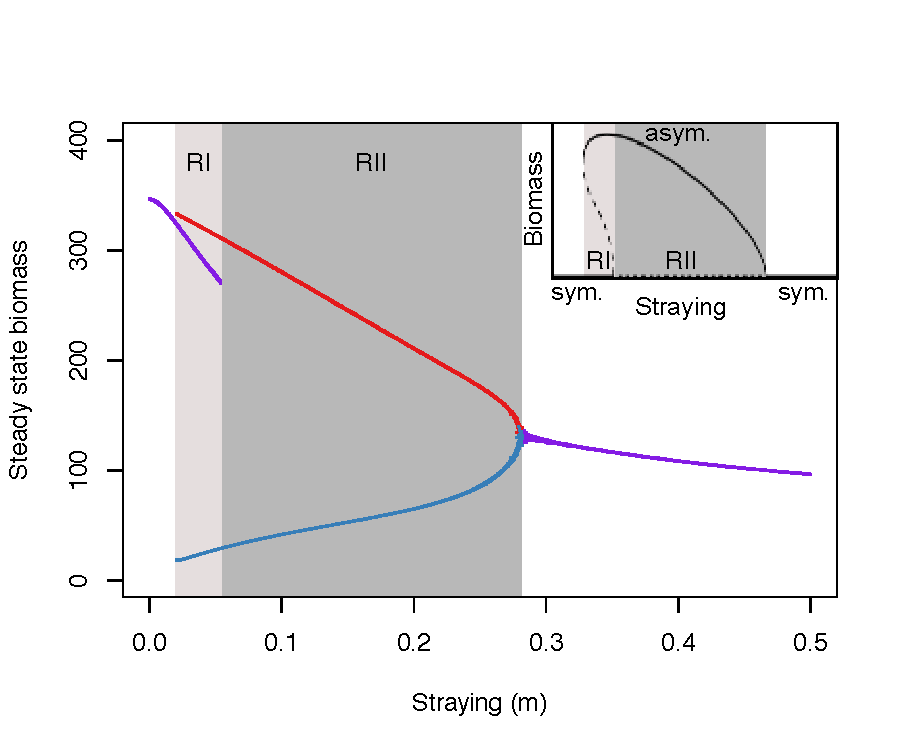
\includegraphics[width=0.75\textwidth]{fig_traj2.pdf}
\caption{
% The steady-state densities of $N_i$ and $N_j$ vs. straying $m$ for the constant straying model. 
% Alternative stable states exist for regimes I and II, labeled RI and RII, respectively.
% Two configurations exist in regime I: a symmetric, intermediate state (solid line), and an asymmetric dominant/subordinate state (red and blue dashed lines, respectively).
% One configuration exists in regime II: an asymmetric dominant/subordinate state (red and blue lines, respectively).
% Inset: An illustration of the alternative stable states (solid lines) in regime I (light gray area) and II (dark gray area).
% The dividing line that separates initial conditions that approach the symmetric (sym.) and asymmetric (asym.) solution is a separatrix (dashed line) that runs through an unstable fixed point.
The steady-state densities of $N_i$ and $N_j$ vs.~straying $m$ for the constant straying model. 
Alternative stable states exist for regimes I and II, labeled RI and RII, respectively. 
In regime I the system can approach qualitatively different states: a symmetric, intermediate state (purple points), and asymmetric dominant/subordinate states (red and blue points, respectively). 
In regime II only one type of attractor exists: an asymmetric dominant/subordinate state (red and blue points, respectively), and its mirror image where identities of dominant and subordinate are exchanged.
Inset: A qualitative sketch of the bifurcation diagram, showing the stable (solid lines) and unstable (dashed line) fixed points in regime I (light gray area) and II (dark gray area).
The symmetric condition (sym.) is the horizontal line at the base of the inset, whereas the asymmetric condition (asym.) is represented by the curved line.
} \label{fig:traj}
\end{figure}


\begin{figure*}
  \captionsetup{justification=raggedright,
singlelinecheck=false
}
\centering
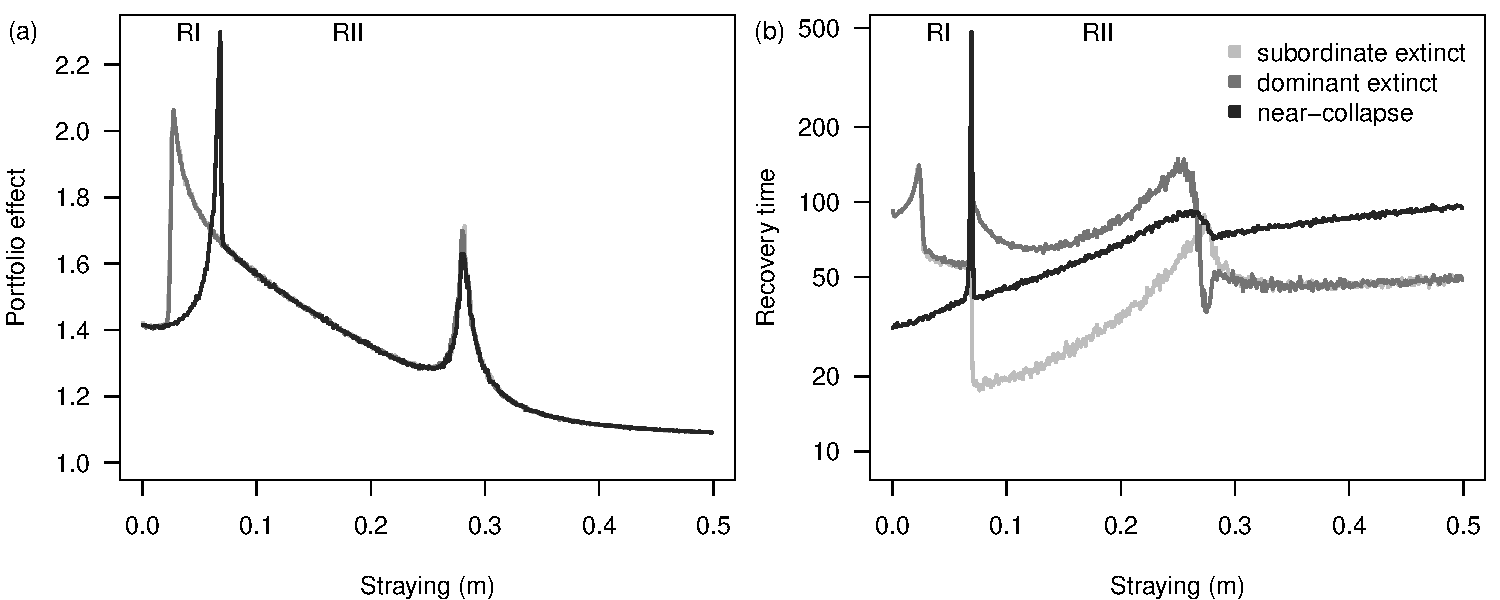
\includegraphics[width=1\textwidth]{fig_mpert.pdf}
\caption{
Measures of metapopulation robustness for the constant straying model as a function of straying $m$.
Alternative stable state regimes I and II corresponding to those in figure \ref{fig:traj} are labeled RI and RII, respectively.
(a) Portfolio effect as a function of $m$.
(b) Recovery time as a function of $m$.
Measures of metapopulation robustness are shown with respect to different induced disturbances: the near-collapse of both populations (black), and the lone extinction of either the dominant (dark gray) or subordinate (light gray) population.
Portfolio effects are different for the near-collapse and single extinction scenarios due to different CVs for the populations and aggregate in alternative basins of attraction that exist in regimes I and II.
} \label{fig:mpert}
\end{figure*}


\begin{figure*}
  \captionsetup{justification=raggedright,
singlelinecheck=false
}
\centering
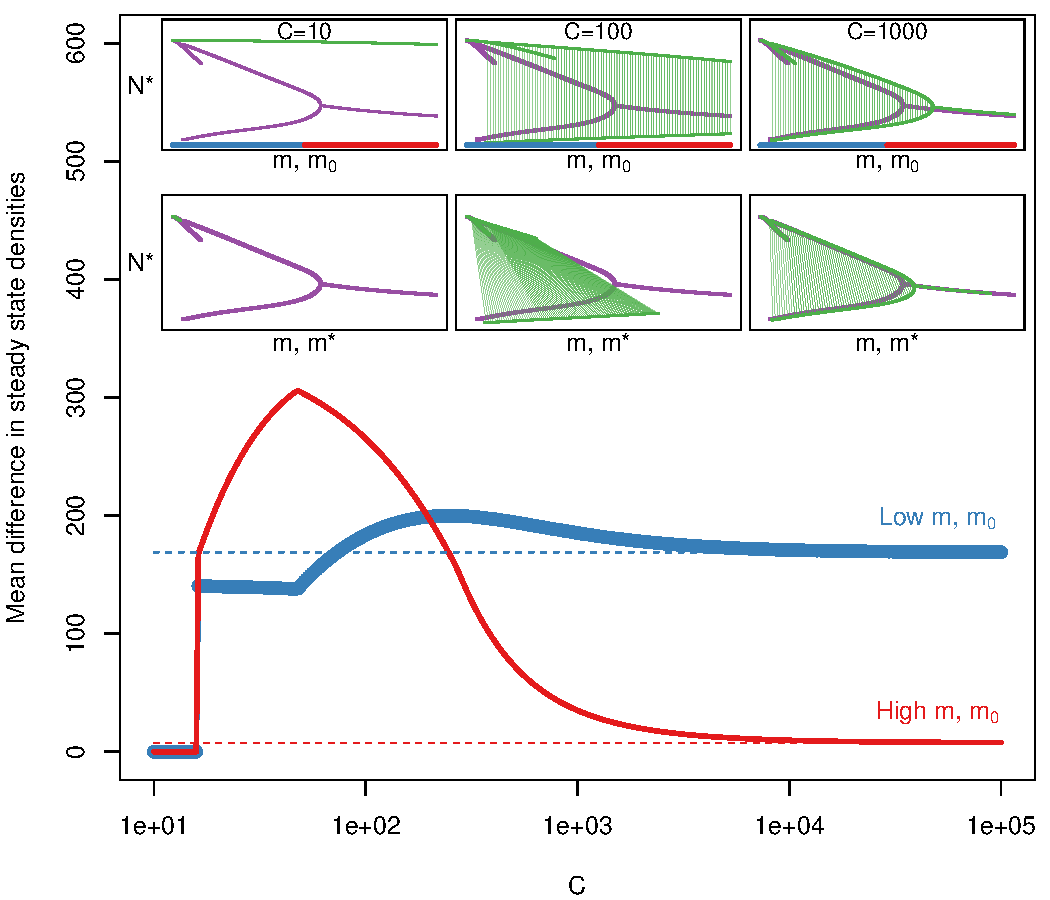
\includegraphics[width=0.75\textwidth]{fig_meandiff2.pdf}
\caption{
Comparison of steady state population densities for the constant straying model and density-dependent straying model.
Inset: stable state densities for the constant straying model (purple) and density-dependent straying model (green) for different strengths of collective behaviour.
Low $C$ corresponds to strong effects of collective behaviour.
The top row shows stable state densities as a function of individual straying $m_0$; the bottom row shows stable state densities as a function of straying at the stable state $m(t)^*$.
Vertical green lines link paired subordinate and dominant population densities.
Main: The absolute difference in stable state densities averaged across intervals of low straying ($0 < m,m_0 < 0.25$; blue) and high straying ($0.25 < m,m_0 < 0.5$; red).
} \label{fig:cb}
\end{figure*}


\begin{figure*}
  \captionsetup{justification=raggedright,
singlelinecheck=false
}
\centering
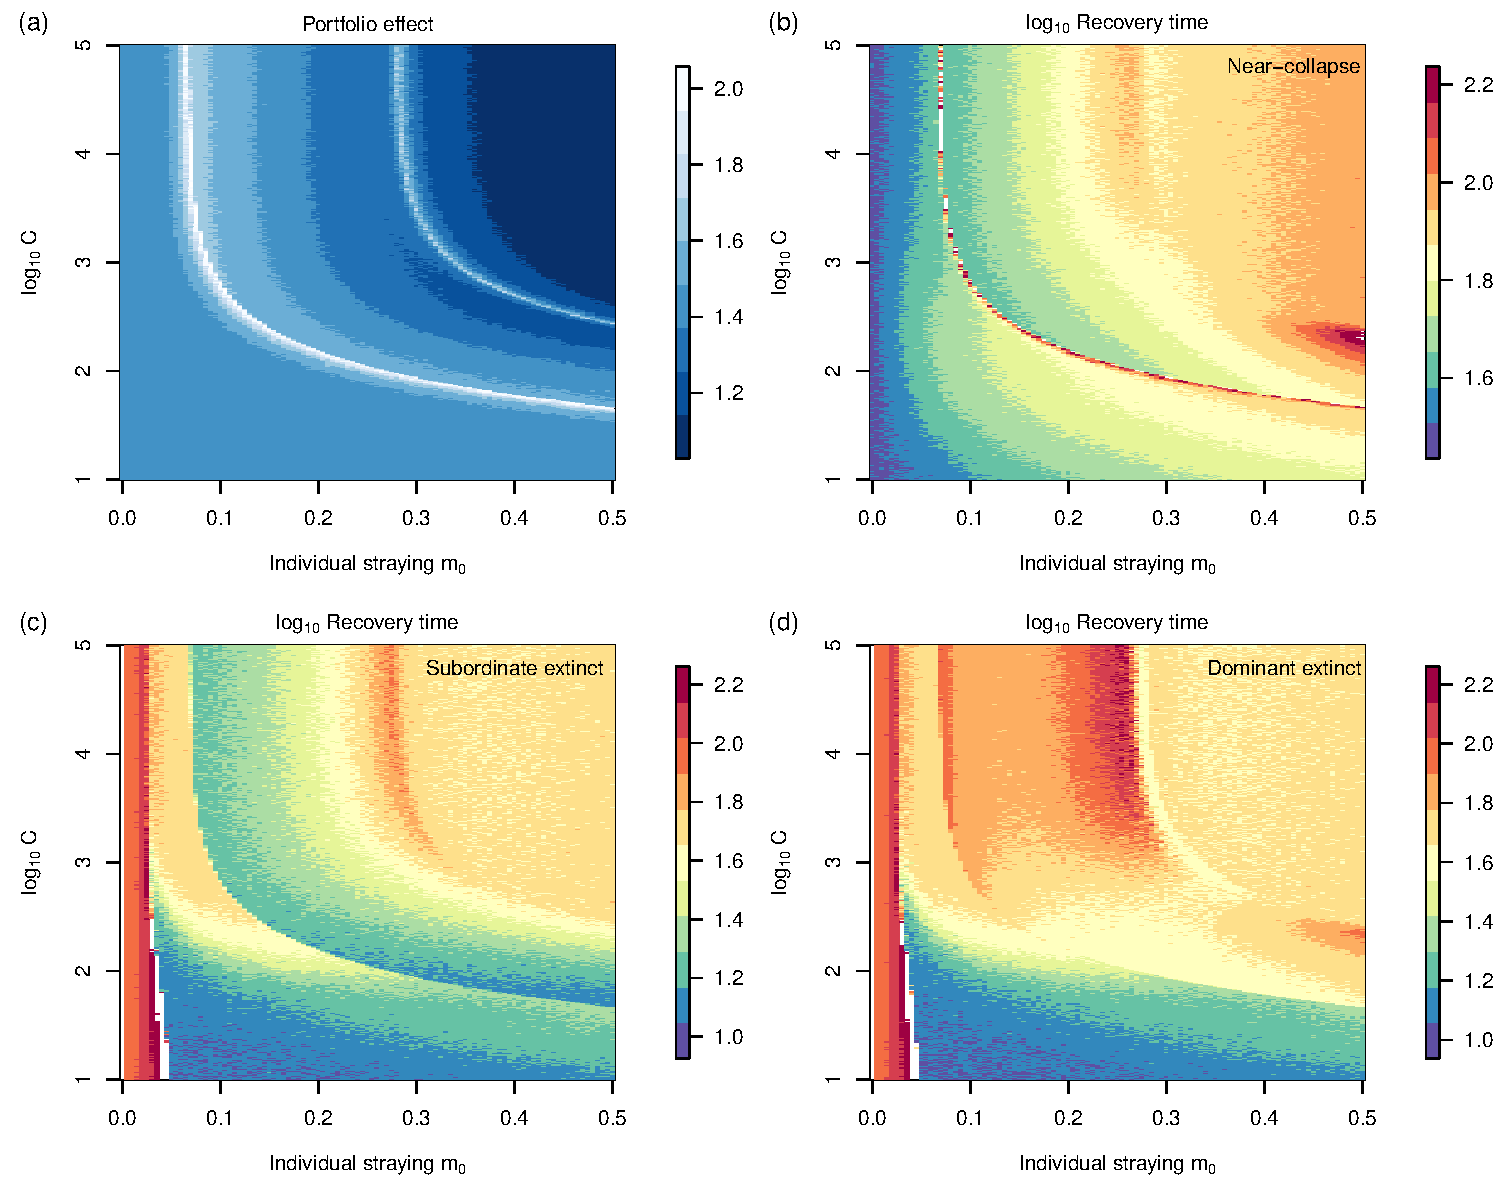
\includegraphics[width=0.75\textwidth]{fig_rtpe_ddm.pdf}
\caption{
Measures of metapopulation robustness for the density-dependent straying model as a function of individual straying $m_0$ and the strength of collective behaviour $C$ (note the $\rm log_{10}$ scale, including 
a) the Portfolio effect,
b) the time to recovery following near-collapse of both populations,
c) the time to recovery following the extinction of the subordinate population, and
d) the time to recovery following the extinction of the dominant population.
} \label{fig:pert}
\end{figure*}



\begin{figure*}
  \captionsetup{justification=raggedright,
singlelinecheck=false
}
\centering
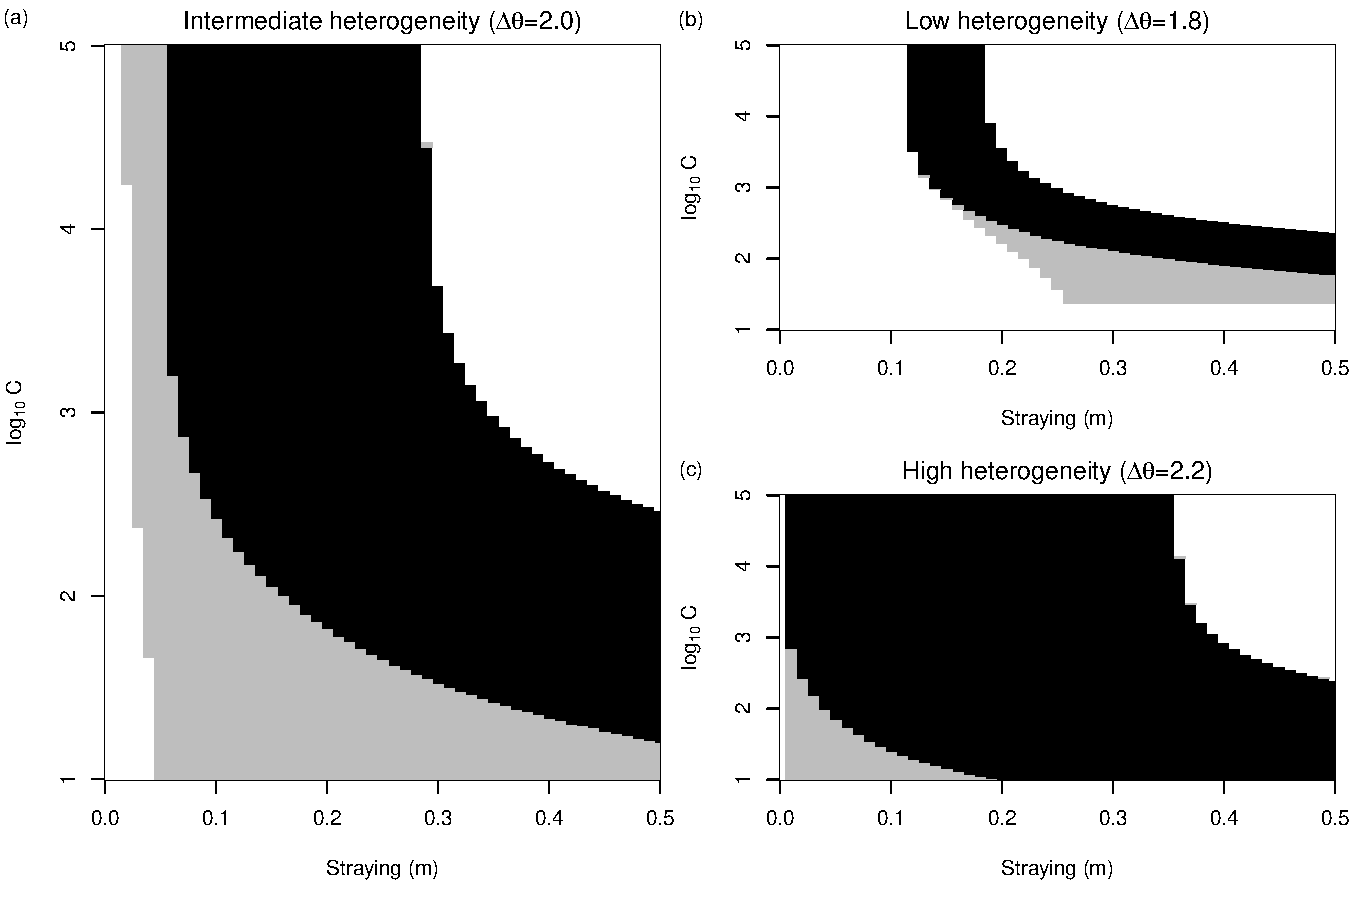
\includegraphics[width=0.75\textwidth]{fig_hysteresis_ddm.pdf}
\caption{
Alternative stable state regimes I (gray) and II (black) as a function of individual straying $m_0$ and the strength of collective behaviour $C$ (note the $\rm log_{10}$ scale).
Regime I signifies parameter space where there is either 1) an intermediate-density, symmetric, steady state, or 2) an asymmetric dominant/subordinate density.
Regime II signifies parameter space where there is an asymmetric dominant/subordinate steady state density.
The white space to the left (lower values of $m_0$) signifies high-density, symmetric, stable states, and the white space to the right (higher values of $m_0$) signifies low-density, symmetric, steady states.
Relationships are shown for (a) intermediate habitat heterogeneity ($\Delta\theta$), as well as (b) low habitat heterogeneity and (c) high heterogeneity.
} \label{fig:bifurcationsddm}
\end{figure*}


\begin{figure*}
  \captionsetup{justification=raggedright,
singlelinecheck=false
}
\centering
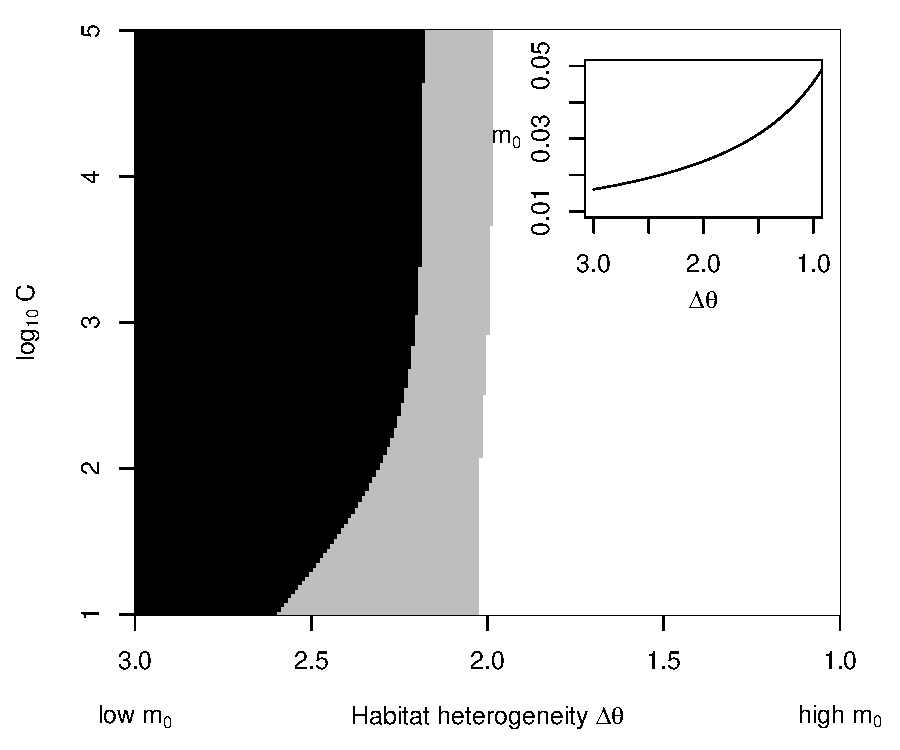
\includegraphics[width=0.5\textwidth]{fig_hysteresis_ddm_mtheta.pdf}
\caption{
Alternative stable state regimes I (gray) and II (black) as a function of individual straying $m_0$ and the strength of collective behaviour $C$ (note the $\rm log_{10}$ scale), for the case where individual straying increases with lower habitat heterogeneity (inset).
Regime I signifies parameter space where there is either 1) an intermediate-density, symmetric, steady state, or 2) an asymmetric dominant/subordinate density.
Regime II signifies parameter space where there is an asymmetric dominant/subordinate steady state density.
} \label{fig:mtheta}
\end{figure*}



%%%%%%%%%%%%%
% SUPPLEMENTARY FIGURES
%%%%%%%%%%%%%

\beginsupplement



\begin{figure}
  \captionsetup{justification=raggedright,
singlelinecheck=false
}
\centering
% 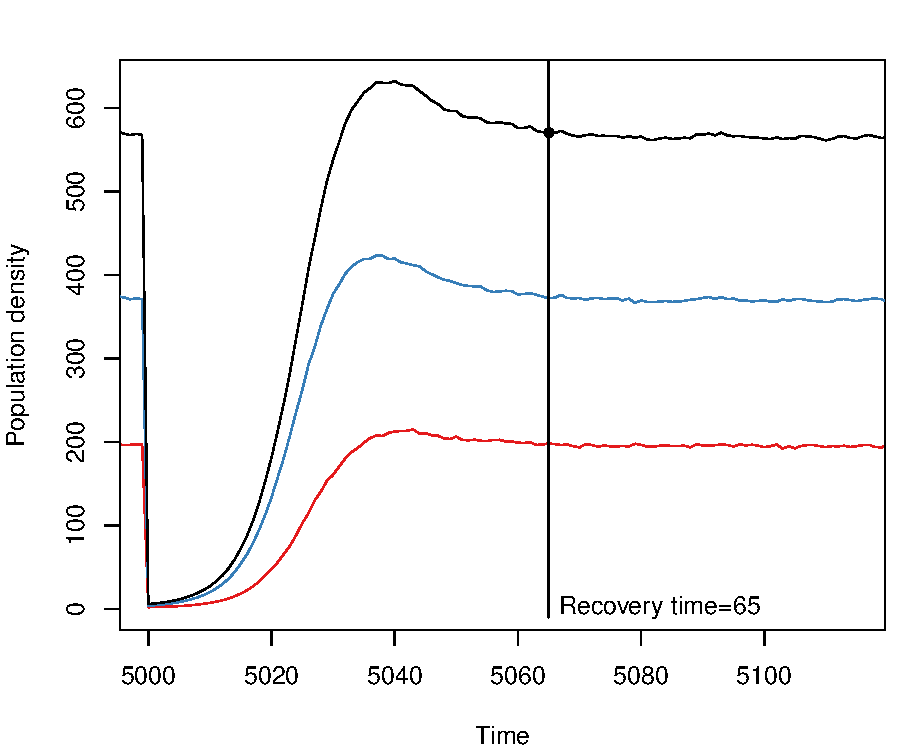
\includegraphics[width=0.35\textwidth]{fig_recovery.pdf}
\caption{
Example of the numerical procedure used to estimate recovery time. After a disturbance is introduced, the recovery time is calculated by measuring the point in time where $N_T$ (in black), which is the aggregate of both populations (blue, red), settles to within one standard deviation of the new equilibrium $N_T^*$. 
} \label{fig:recovery}
\end{figure}



\begin{figure}
  \captionsetup{justification=raggedright,
singlelinecheck=false
}
\centering
% 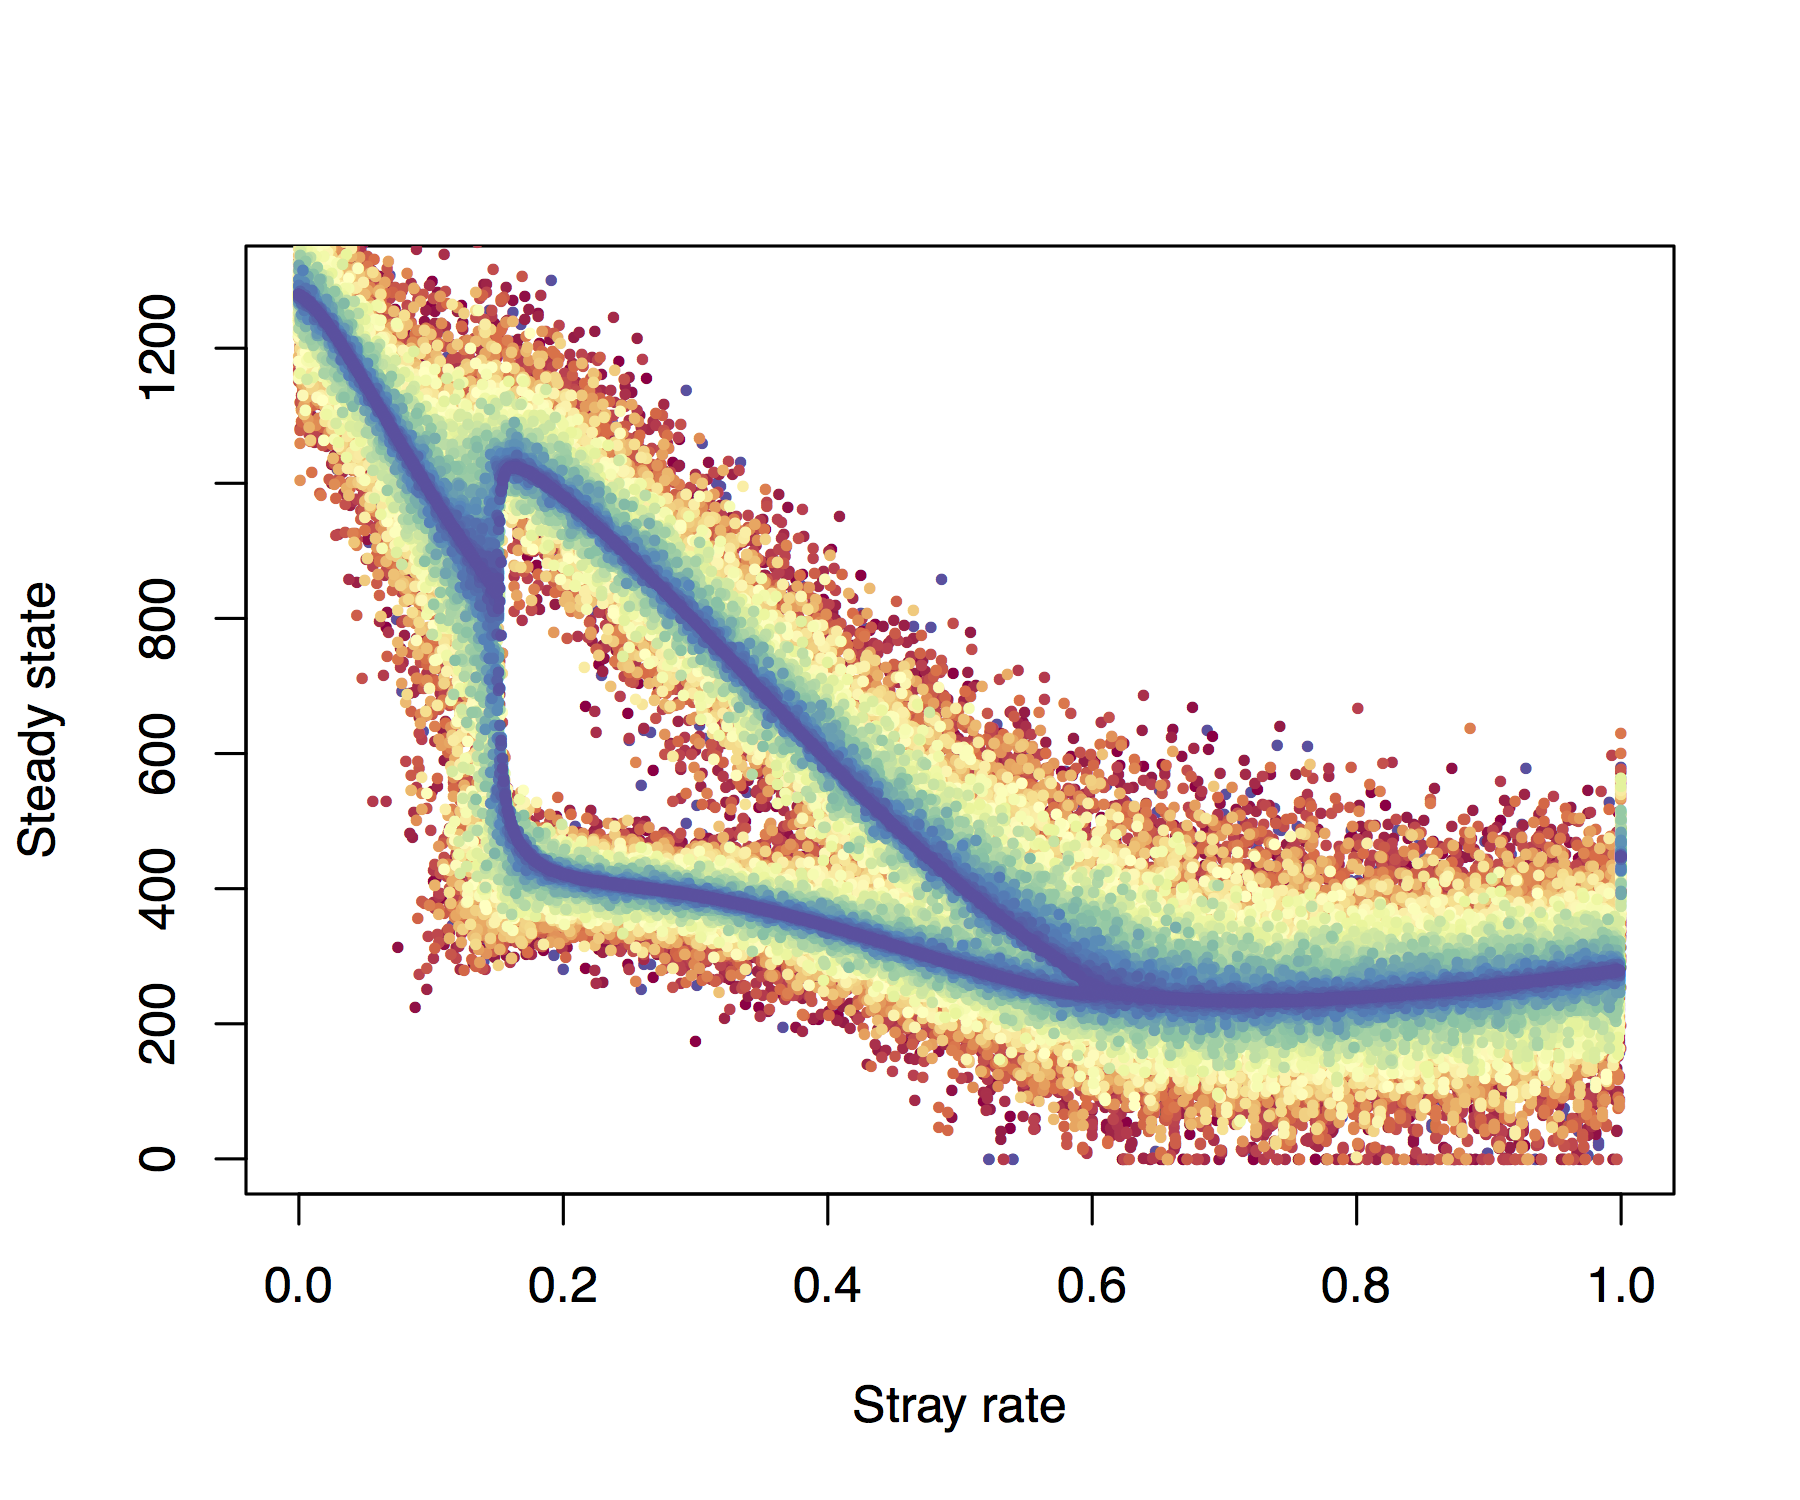
\includegraphics[width=0.35\textwidth]{fig_density.png}
\caption{
Steady-state densities of both populations as a function of $m$: one in a dominant state and one in a subordinate state.
Steady-states for populations with symmetrical values ($\alpha=0$) in the vital rates $r_{\rm max}$ and $\beta$ are shown with cool tones.
As the asymmetry among populations between sites increases ($\alpha>0$), their vital rates diverge, such that the maximal growth at sites 1 and 2 is now $r_{\rm max,1}=(1 + \alpha)r_{\rm max,2}$ and $\beta_1=(1+\alpha)\beta_2$ where $\alpha$ is increased from $0$ to $0.1$, thereby increasing the asymmetry in vital rates.
Steady-states for populations with increasingly asymmetric values ($\alpha\rightarrow 0.1$) for vital rates $r_{\rm max}$ and $\beta$ are shown in warmer tones.
The lower-density values that appear between $m=0.06$ and $m=0.1$ represent populations that have been trapped in the low-density basins of attraction associated with regime I.
Increasing the asymmetry in vital rates does not impact the qualitative nature of the dynamics.
} \label{fig:symmetry}
\end{figure}




\begin{figure}
  \captionsetup{justification=raggedright,
singlelinecheck=false
}
\centering
% 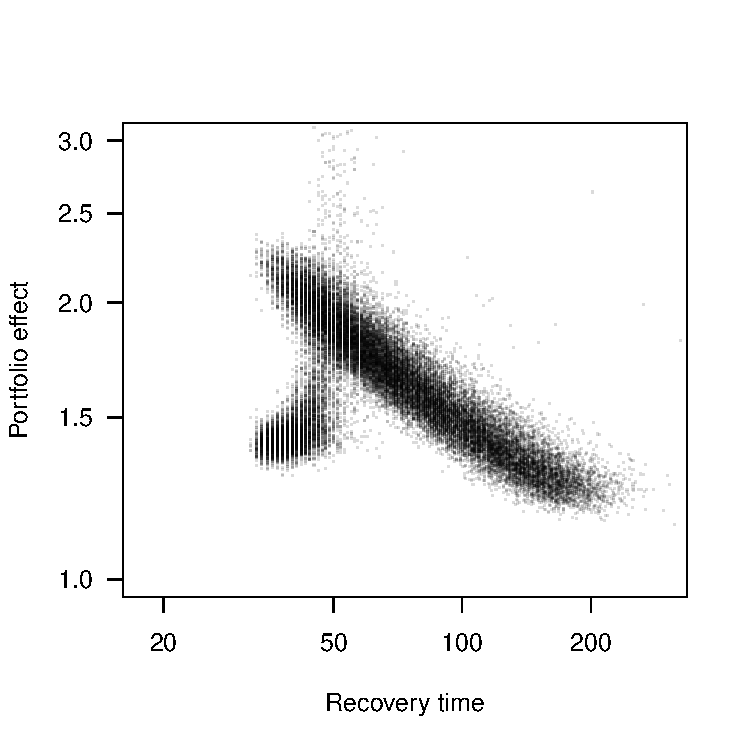
\includegraphics[width=0.35\textwidth]{fig_pevsrt.pdf}
\caption{
Comparison of portfolio effects vs. recovery time following the near-collapse of both populations.
} \label{fig:pevsrt}
\end{figure}






\end{document}
